\documentclass[slidetop,11pt]{beamer}
%
% Ces deux lignes {\`a} d{\'e}commenter pour sortir 
% le texte en classe article
% \documentclass[class=article,11pt,a4paper]{beamer}
% \usepackage{beamerbasearticle}

% Packages pour les fran\c{c}ais
%
\usepackage[T1]{fontenc} 
\usepackage[latin1]{inputenc}
\usepackage[frenchb]{babel}
% pour un pdf lisible {\`a} l'{\'e}cran si on ne dispose pas 
% des fontes cmsuper ou lmodern
%\usepackage{lmodern}
\usepackage{aeguill}

% Pour afficher le pdf en plein ecran
% (comment{\'e} pour imprimer les transparents et pour les tests)
%\hypersetup{pdfpagemode=FullScreen}

% ------------------------------------------------
%-----------   styles pour beamer   --------------
% ------------------------------------------------
%
% ------------- Choix des couleurs ---------------

%% %% %% %% %% COULEURS PERSOS
\definecolor{verylightblack}{rgb}{0.25,0.25,0.25}
\definecolor{lightblack}{rgb}{0.1,0.1,0.1}
\definecolor{black}{rgb}{0,0,0}


\definecolor{verylightgrey}{rgb}{0.8,0.8,0.8}
\definecolor{lightgrey}{rgb}{0.6,0.6,0.6}
\definecolor{grey}{rgb}{0.4,0.4,0.4}

\definecolor{verylightgray}{gray}{0.80}
\definecolor{lightgray}{gray}{0.6}
\definecolor{gray}{gray}{0.4}

\definecolor{verylightblue}{rgb}{0.9,0.9,1.0}
\definecolor{lightblue}{rgb}{0.75,0.75,1.0}
\definecolor{blue}{rgb}{0.5,0.5,1.0}
\definecolor{darkblue}{rgb}{0.0,0.0,0.5}

\definecolor{verylightred}{rgb}{1.0,0.9,0.9}
\definecolor{lightred}{rgb}{1.0,0.75,0.75}
\definecolor{red}{rgb}{1.0,0.5,0.5}

\definecolor{verylightgreen}{rgb}{0.9,1.0,0.9}
\definecolor{lightgreen}{rgb}{0.75,1.0,0.75}
\definecolor{green}{rgb}{0.5,1.0,0.5}


\definecolor{verylightcolorGREY}{gray}{0.80}
\definecolor{lightcolorGREY}{gray}{0.60}

\definecolor{verylightcolorRED}{rgb}{1.0,0.9,0.9}
\definecolor{lightcolorRED}{rgb}{1.0,0.75,0.75}

\definecolor{verylightcolorUN}{rgb}{1.0,0.75,1.0}
\definecolor{lightcolorUN}{rgb}{1.0,0.50,1.0}

\definecolor{verylightcolorDE}{rgb}{0.75,1.0,1.0}
\definecolor{lightcolorDE}{rgb}{0.50,1.0,1.0}

\definecolor{verylightcolorTR}{rgb}{1.0,1.0,0.75}
\definecolor{lightcolorTR}{rgb}{1.0,1.0,0.50}


% Red{\'e}finit la couleur de fond pour imprimer sur transparents
%\xdefinecolor{fondtexte}{rgb}{1,1,1}     % blanc

% commande differente pour les couleurs nomm{\'e}es - de base
%\colorlet{coultexte}{black} 

% -------------- Fioritures de style -------------
% Fait afficher l'ensemble du frame 
% en peu lisible (gris clair) d{\`e}s l'ouverture
\beamertemplatetransparentcovered

% Supprimer les icones de navigation (pour les transparents)
%\setbeamertemplate{navigation symbols}{}

% Mettre les icones de navigation en mode vertical (pour projection)
%\setbeamertemplate{navigation symbols}[vertical]

% ------------ Choix des th{\`e}mes ------------------
\usecolortheme{default} % gabywald
% \usecolortheme{orchid}

\setbeamercolor{title}{fg=black, bg=red!40}
\setbeamercolor{block title}{fg=black, bg=red!40}
\setbeamercolor{structure}{fg=black, bg=red!40}
\setbeamercolor{block title}{fg=black, bg=lightred!40}
\setbeamercolor{substructure}{fg=black, bg=verylightred!40}

\setbeamercolor{block title GREY}{fg=black, bg=lightcolorGREY!40}
\setbeamercolor{substructureGREY}{fg=black, bg=verylightcolorGREY!40}

\setbeamercolor{block title RED}{fg=black, bg=lightcolorRED!40}
\setbeamercolor{substructureRED}{fg=black, bg=verylightcolorRED!40}

\setbeamercolor{block title UN}{fg=black, bg=lightcolorUN!40}
\setbeamercolor{substructureUN}{fg=black, bg=verylightcolorUN!40}

\setbeamercolor{block title DE}{fg=black, bg=lightcolorDE!40}
\setbeamercolor{substructureDE}{fg=black, bg=verylightcolorDE!40}

\setbeamercolor{block title TR}{fg=black, bg=lightcolorTR!40}
\setbeamercolor{substructureTR}{fg=black, bg=verylightcolorTR!40}

% \setbeamercolor{block title}{fg=black, bg=lightblue!40}
% \setbeamercolor{block body}{...}
% \setbeamercolor{block title example}{...}
% \setbeamercolor{block body example}{...}
% \setbeamercolor{block title alerted}{...}
% \setbeamercolor{block body alerted}{...}

% \useoutertheme[left]{sidebar}
% \setbeamersize{sidebar left width=3.0cm \tableofcontents[hideothersubsections] }
% \setbeamercolor{sidebar left}{fg=green,bg=lightgreen}
% \setbeamercolor{title in sidebar}{parent=title}

\setbeamercolor*{sidebar}{fg=lightblack,bg=lightblue!75!white}

\setbeamercolor*{palette sidebar primary}{fg=darkblue!50!lightgrey}
\setbeamercolor*{palette sidebar secondary}{fg=black} % darkblue!10!black
\setbeamercolor*{palette sidebar tertiary}{fg=darkblue!50!lightgrey}
\setbeamercolor*{palette sidebar quaternary}{fg=black} % darkblue!10!black

% \setbeamercolor{subsubsection in sidebar}{hideallsubsections}
% \setbeamercolor{subsubsection in sidebar shaded}{hideallsubsections}


%------------ fin style beamer -------------------

% Faire appara{\^i}tre un sommaire avant chaque section
% \AtBeginSection[]{
%   \begin{frame}
%   \frametitle{Plan}
%   \medskip
%   %%% affiche en d{\'e}but de chaque section, les noms de sections et
%   %%% noms de sous-sections de la section en cours.
%   \small \tableofcontents[currentsection, hideothersubsections]
%   \end{frame} 
% }

% ----------- Contenu de la page de titre --------
\title{La Ligue Ludique Pr{\'e}sente : }
\subtitle{ARG : Alternate Reality Game / Jeu en R{\'e}alit{\'e} Altern{\'e}e (JRA) \newline Jeux TransM{\'e}dias}
% \author{Gabriel Chandesris & Florent Touzeau-Genty}
% \institute{Universit{\'e} de Barrayar}
\institute{
\includegraphics[width=5cm]{img/ligueludique-1.png}}
\date{\today} %% \date{08 Novembre 2010}
%% \logo{
\includegraphics[height=0.5cm]{img/logo_glider.png}}

% ----------- Notes plan vu AmaelAssour + DaftFlo le 201702041500-1700 --------

%% Quelques noms / exemples de ARG / JRA
%% %% Perplex City
%% %% The Beast (_Artificial Intelligence_)
%% %% Tron Legacy / Super 8 / ...
%% %% The Lost Experience
%% %% The Lost Ring
%% %% Majestic
%% %% William Gibson ?
%% %% _Ceci n'est pas un jeu_ (Walter Jon Williams)
%% %% "The Web Soap" (comme exemple de Proto-ARG)
%% Principes +/- g{\'e}n{\'e}raux, reprise {\`a} partir des exemples
%% %% transmedia : raconter une histoire / fiction en changeant de m{\'e}dia (continuit{\'e} de l'histoire)
%% %% Chasse au tr{\'e}sor : trouver les indices, interragir avec les protagonistes (en-ligne voire IRL), comment acc{\'e}der aux indices ?!
%% %% Utilisation d'InterNet (blogs, r{\'e}seaux sociaux...), essentiellement Web accessible / grand public
%% %% => accessible {\`a} la curiosit{\'e} de tout un chacun ("le spectateur est-il curieux ?" cf. s{\'e}rie TV Lost et ARG associ{\'e})
%% %% => diff{\'e}rents publics distincts (au moins deux)
%% Gros formats => Grosses boites (mais ne veut pas dire grosse audience)
%% %% Petits, moins diffus{\'e}s, mais public cible / cibl{\'e} !
%% %% Communaut{\'e} cach{\'e} / "secr{\`e}te", int{\'e}r{\^e}t pour les {\'e}nigmes, l'aspect "romanesque" sur les r{\'e}seaux informatiques (avant tout !) mais un lien entre le r{\'e}el et le virtuel (une flash mob, une rencontre IRL entre joueurs...)

%% Pourquoi faire un ARG ?
%% %% Promouvoir un {\'e}v{\`e}nement
%% %% Promouvoir un {\'e}l{\'e}ment commercial ponctuel (film, jeu vid{\'e}o...) qui auto-alimente le jeu ?!
%% %% Loisir / culture / tourisme (visite d'un mus{\'e}e par exemple ou d'un lieu d'int{\'e}r{\^e}t)

%% Parall{\`e}le avec le JdR / Jeu de R{\^o}le
%% %% Histoire / sc{\'e}nario
%% %% MJ / {\'e}quipe derri{\`e}re (beaucoup plus cach{\'e})

% ----------- Nom des diff{\'e}rentes parties --------

%% Mis au fur et {\`a} mesure...

\def\moreInFrameTitleLeftt{
\includegraphics[height=0.5cm]{img/ligueludique-0.png}~~~~~}
\def\moreInFrameTitleRight{~~~~~
\includegraphics[height=0.5cm]{img/logo_glider.png}}

% ------------------------------------------------
% -------------   D{\'e}but document   ---------------
% ------------------------------------------------
\begin{document}
%--------- {\'e}criture de la page de titre ----------
% avec la commande frame simplifi{\'e}e
\frame[plain]{\titlepage}
%

%------------------ Sommaire ---------------

\begin{frame}
	\frametitle{\moreInFrameTitleLeftt Sommaire \moreInFrameTitleRight}
	\small \tableofcontents[hideallsubsections]
\end{frame} 


%***************************************
%******     I Pr{\'e}sentation  *******
%***************************************
\def\sectionPartI{Pr{\'e}sentation de la Ligue Ludique}
\section{\sectionPartI}
\begin{frame}
	\frametitle{\moreInFrameTitleLeftt \sectionPartI}
	\tableofcontents[sections=1,currentsection,subsectionstyle=show/shaded/hide] %% sectionstyle=hide/hide,
\end{frame} 

\def\sectionPartIa{La Ligue Ludique}
\subsection{\sectionPartIa}
\begin{frame}
	\frametitle{\moreInFrameTitleLeftt \sectionPartIa}
	\tableofcontents[sections=1,currentsection,subsectionstyle=show/shaded/hide]
\end{frame}

\def\sectionPartIaUN{Ligue Ludique... Jeux de R{\^o}le ! }
\subsubsection{\sectionPartIaUN}
\begin{frame}
	\frametitle{\moreInFrameTitleLeftt \sectionPartIaUN}
	\begin{columns}[T]
		\begin{column}[T]{3.5cm}
			
\includegraphics[height=3.4cm]{img/ligueludique-1.png} %% {img/omnesDOCETubique.png}
		\end{column}
		\begin{column}[T]{7cm}
			 \begin{beamerboxesrounded}	[lower=substructureRED, %
							 upper=block title RED,%
							 shadow=true]%
				   {\sectionPartIaUN}
				\begin{itemize}
					\item Association loi 1901, fond{\'e}e en 2008, 
					\item Promotion du JdR (Jeu de R{\^o}le) sur Paris et proche banlieue, 
					\item Parties ouvertes au format court en semaine, 
					\item Partenariats (boutiques, caf{\'e}s...), 
					\item Conventions, salons, {\'e}v{\`e}nements... 
					\item $\Rightarrow$ \underline{\textbf{http://www.ligue-ludique.fr}} $\Leftarrow$
					\item ...
				\end{itemize}
			\end{beamerboxesrounded}
		\end{column}
	\end{columns}
\end{frame}

% ***************************************
% ******     II Th{\'e}matique  	*******
% ***************************************

\def\sectionPartII{ARG -- Alternate Reality Games}
\section{\sectionPartII}
\begin{frame}
	\frametitle{\moreInFrameTitleLeftt \sectionPartII}
	\tableofcontents[sections=2,currentsection,subsectionstyle=show/shaded/hide] %% sectionstyle=hide/hide,
\end{frame} 

\def\sectionPartIIa{Quelques noms}
\subsection{\sectionPartIIa}
\begin{frame}
	\frametitle{\moreInFrameTitleLeftt \sectionPartIIa }
	\tableofcontents[sections=2,currentsection,subsectionstyle=show/shaded/hide]
\end{frame} 

%% \def\sectionPartIIaI{Perplex City}
%% \subsubsection{\sectionPartIIaI}
%% \begin{frame}
%% 	\frametitle{\moreInFrameTitleLeftt \sectionPartIIaI }
%% 	\begin{itemize}
%% 		\item \textbf{ \sectionPartIIaI }
%% 		\item[] ...
%% 		\item \textcolor{red}{ \textbf{TODO} }
%% 	\end{itemize}
%% \end{frame} 

\def\sectionPartIIaII{The Beast \& ... }
\subsubsection{\sectionPartIIaII}
\begin{frame}
	\frametitle{\moreInFrameTitleLeftt \sectionPartIIaII }
	\begin{itemize}
		%% \item \textbf{ \sectionPartIIaII }
		\item ARG associ{\'e}s {\`a} des films (respectivement \emph{Artificial Intelligence} et films {\'e}ponymes tels que \emph{Tron Legacy}, \emph{Super 8}, \emph{Blair Witch}...), 
		\item R{\'e}f{\'e}rences indirectes, marketing indirect, {\'e}l{\'e}ments du g{\'e}n{\'e}rique accessibles sur internet (faux sites web notamment), 
		\item Surtout li{\'e}s aux concepts manipul{\'e}s (Th{\'e}rapies pour Machines Intelligentes, Sorcellerie...). 
	\end{itemize}
\end{frame} 

\def\sectionPartIIaIII{The Lost Experience}
\subsubsection{\sectionPartIIaIII}
\begin{frame}
	\frametitle{\moreInFrameTitleLeftt \sectionPartIIaIII }
	\begin{itemize}
		%% \item \textbf{ \sectionPartIIaIII }
		\item En parall{\`e}le de la s{\'e}rie T{\'e}l{\'e}vis{\'e}e \emph{Lost} (des rescap{\'e}s d'un accident d'avion), 
		\item {\`A} partir de la saison 6, on {\'e}t{\'e} notamment inclus des fausses publicit{\'e}s (\emph{DHARMA initiative), \emph{Hanso Foundation}...} et des (faux) sites web d{\'e}di{\'e}s {\`a} des {\'e}l{\'e}ments r{\'e}currents de la s{\'e}rie TV (\emph{The Valenzetti Equation}), 
		\item Compl{\'e}tait la s{\'e}rie dans un aspect \emph{transmedia}, mais n'a f{\'e}d{\'e}r{\'e} qu'une petite partie des spectateurs de la s{\'e}rie...
	\end{itemize}
\end{frame} 

\def\sectionPartIIaIV{The Lost Ring}
\subsubsection{\sectionPartIIaIV} %% TLR
\begin{frame}
	\frametitle{\moreInFrameTitleLeftt \sectionPartIIaIV  (1) }
	\begin{itemize}
		\item Un beau jour de 2008 (ou une ann{\'e}e bissextile / Olympique / ...), vous recevez un colis Federal Express !
	\end{itemize}
	
	\begin{columns}[T]
		\begin{column}[T]{4.1cm}
			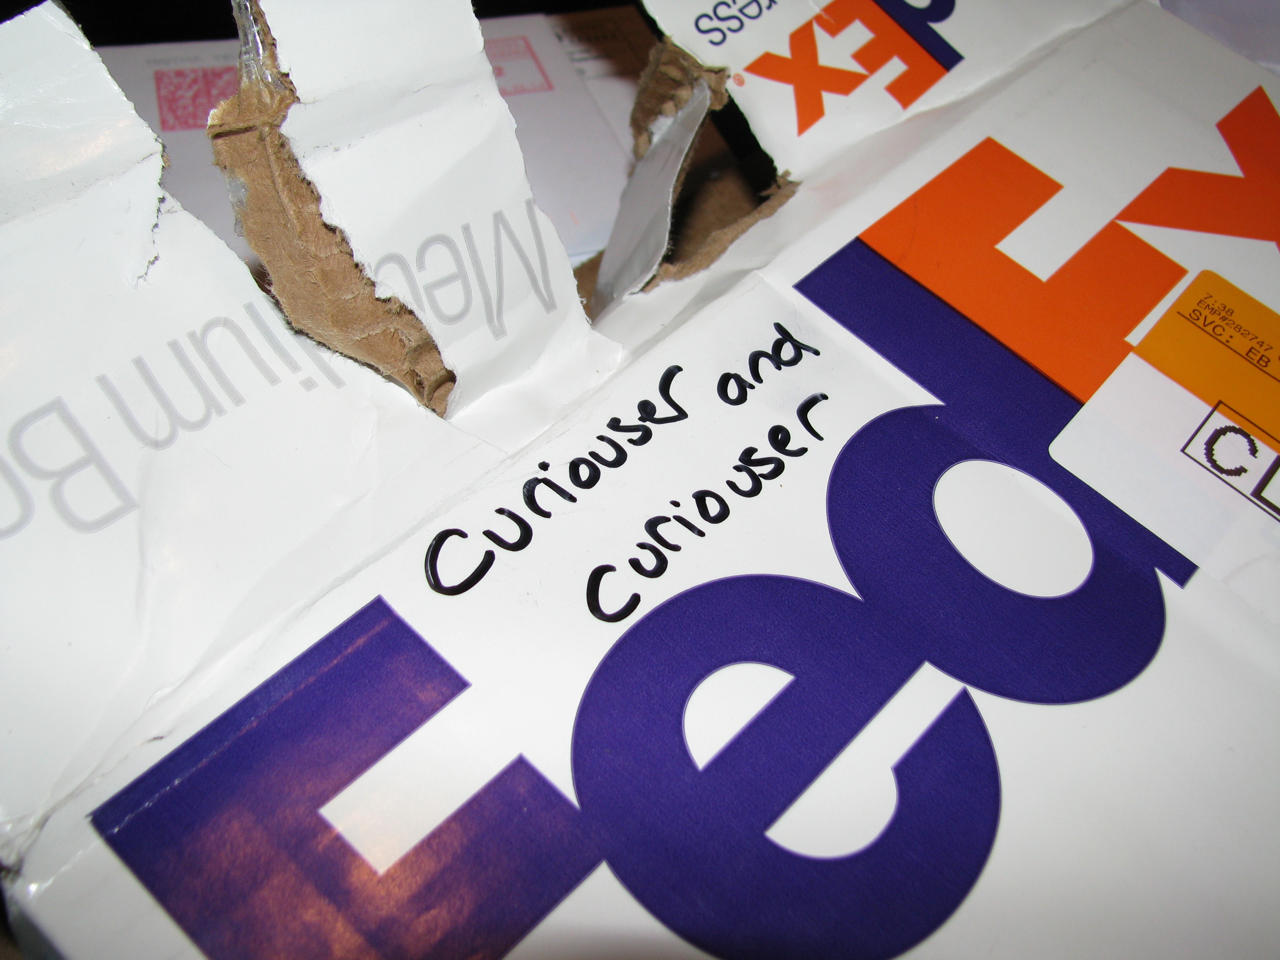
\includegraphics[height=4.05cm]{img/argTheLostRing/2298573987_7e11345d9d_o.jpg}
		\end{column}
		\begin{column}[T]{4.1cm}
			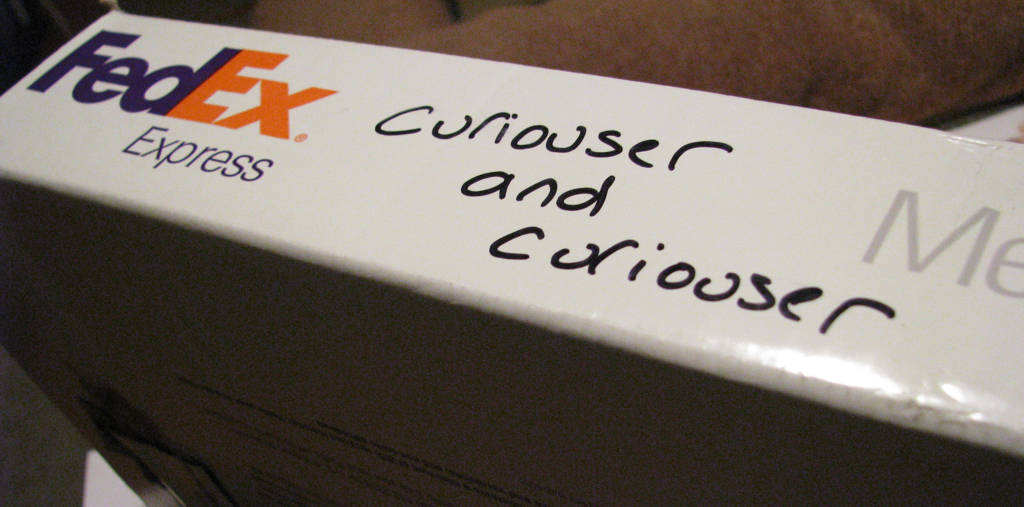
\includegraphics[height=4.05cm]{img/argTheLostRing/2299370570_92295d5e5f_o.jpg}
		\end{column}
		\begin{column}[T]{4.1cm}
			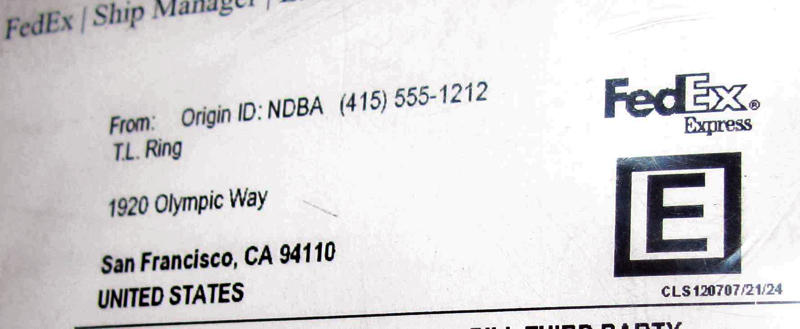
\includegraphics[height=4.05cm]{img/argTheLostRing/2298573877_5b74530a72_o.jpg}
		\end{column}
	\end{columns}
\end{frame} 

\begin{frame}
	\frametitle{\moreInFrameTitleLeftt \sectionPartIIaIV  (2) }
	\begin{itemize}
		\item Un contenu des plus {\'e}trange...
		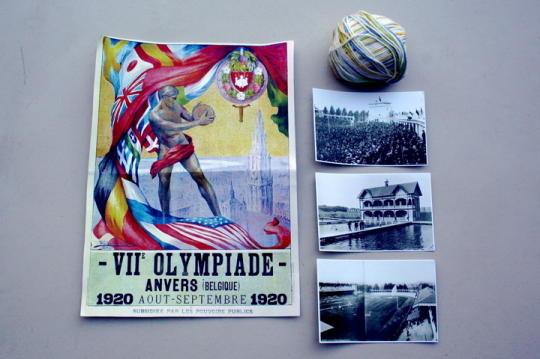
\includegraphics[height=7.00cm]{img/argTheLostRing/Fronts_and_string_540x359.jpg}
	\end{itemize}
\end{frame} 

\begin{frame}
	\frametitle{\moreInFrameTitleLeftt \sectionPartIIaIV  (3) }
	\begin{itemize}
		\item Un poster des Jeux Olympiques de 1920 ?
	\end{itemize}
	\begin{columns}[T]
		\begin{column}[T]{5.05cm}
			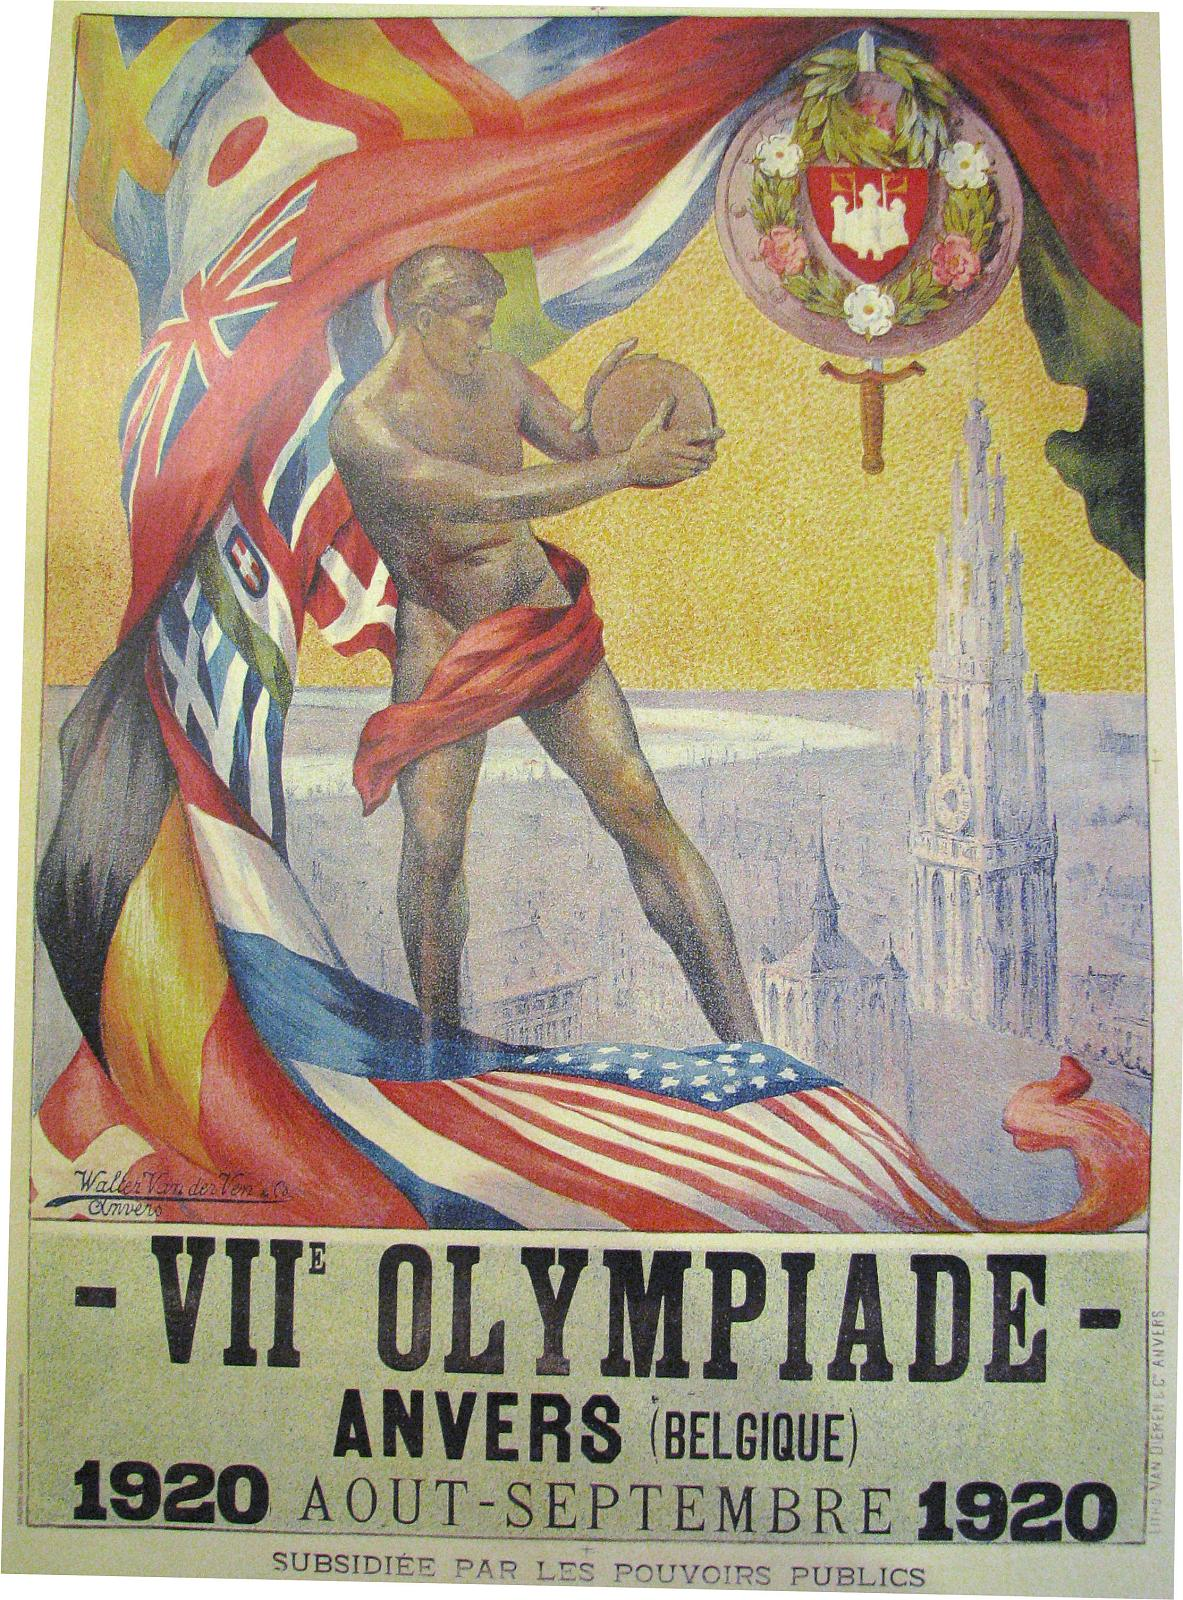
\includegraphics[width=5.00cm]{img/argTheLostRing/2298573863_8f55746c43_o.jpg}
		\end{column}
		\begin{column}[T]{5.05cm}
			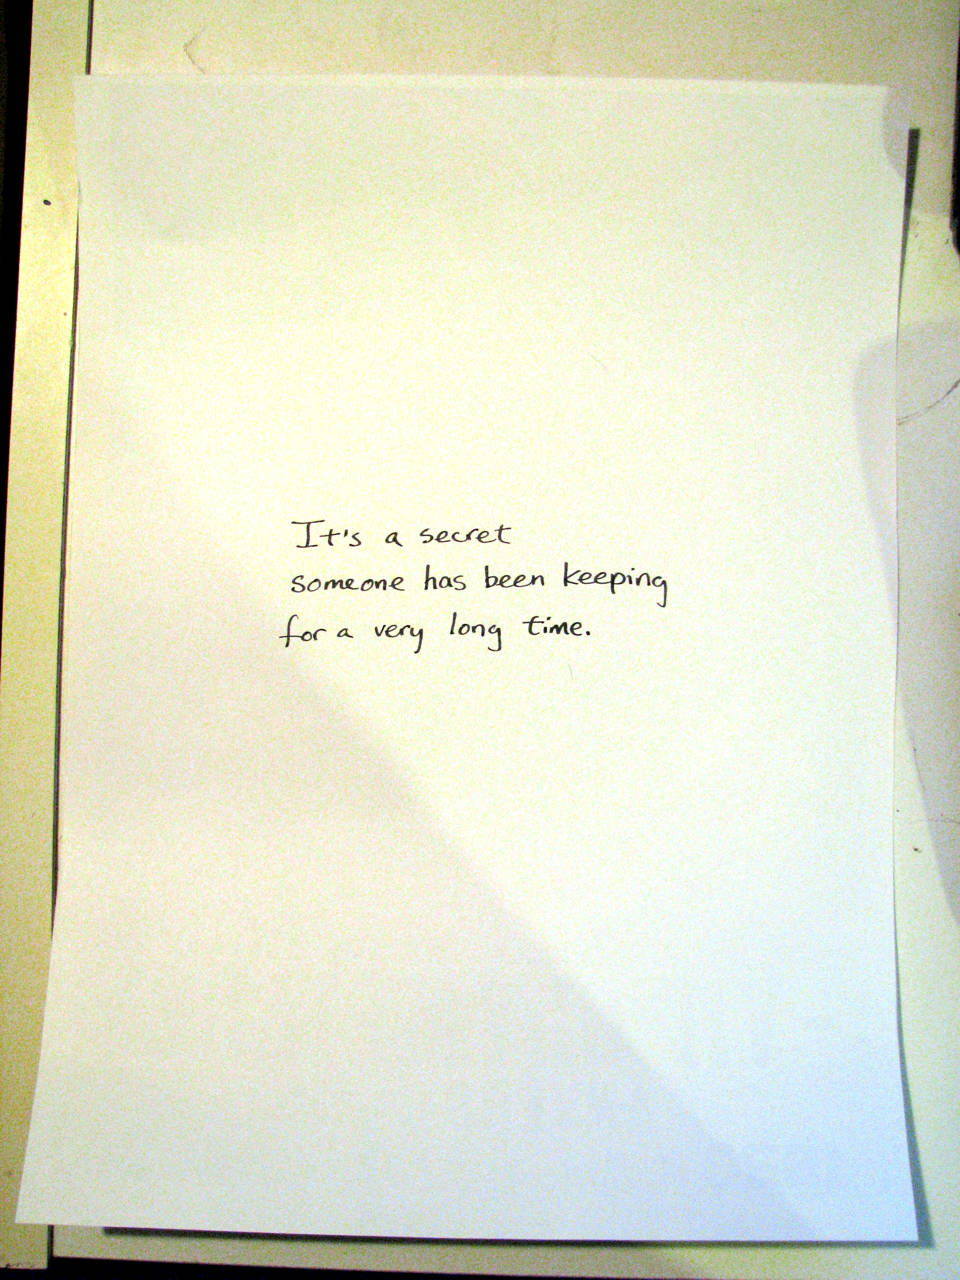
\includegraphics[width=5.00cm]{img/argTheLostRing/2298573691_f5614cb457_o.jpg}
		\end{column}
	\end{columns}
\end{frame} 

\begin{frame}
	\frametitle{\moreInFrameTitleLeftt \sectionPartIIaIV  (4) }
	\begin{itemize}
		\item 3 Cartes Postales Recto-Verso
	\end{itemize}
	\begin{columns}[T]
		\begin{column}[T]{4.05cm}
			%% \item[] Carte Postale 1
			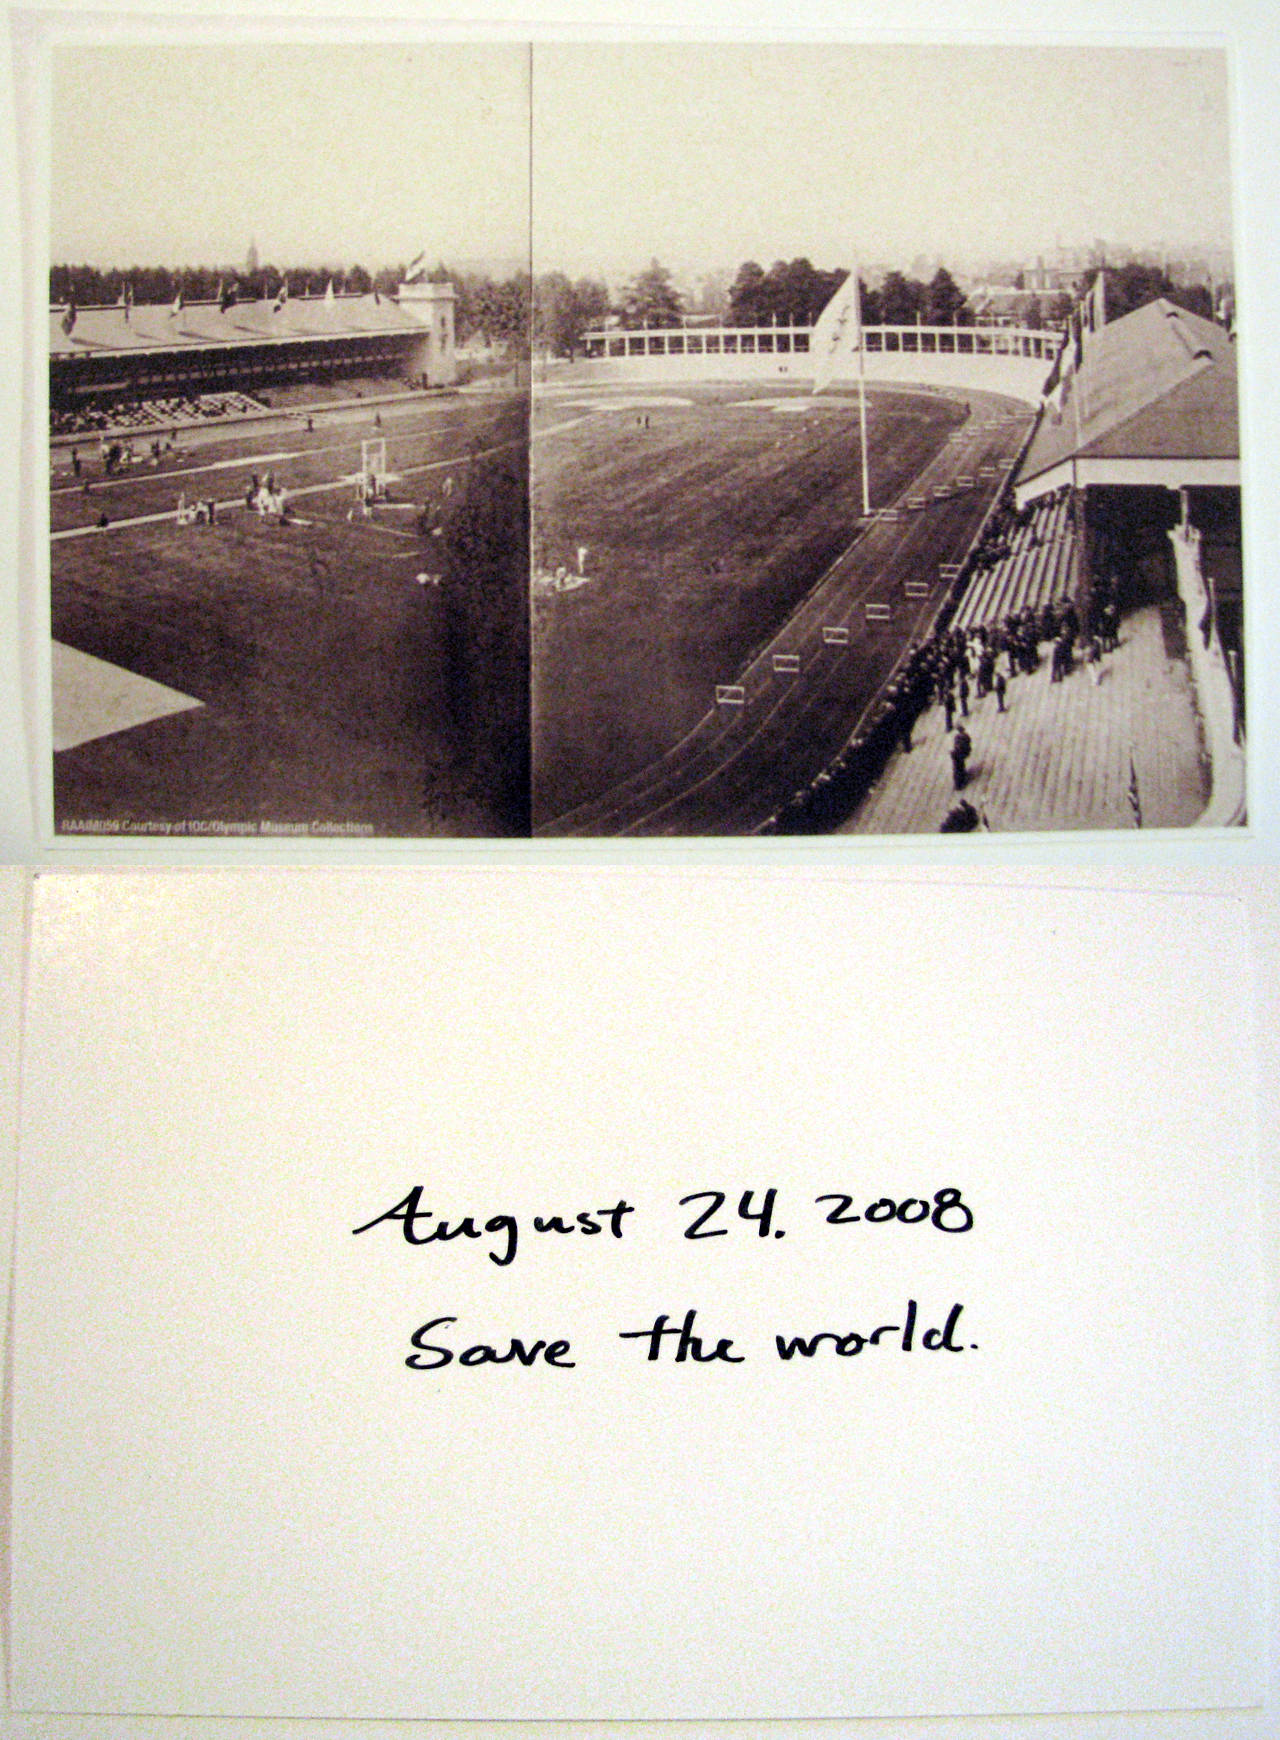
\includegraphics[width=3.95cm]{img/argTheLostRing/2299369980_6cd3e50860_o.jpg}
		\end{column}
		\begin{column}[T]{4.05cm}
			%% \item[] Carte Postale 2
			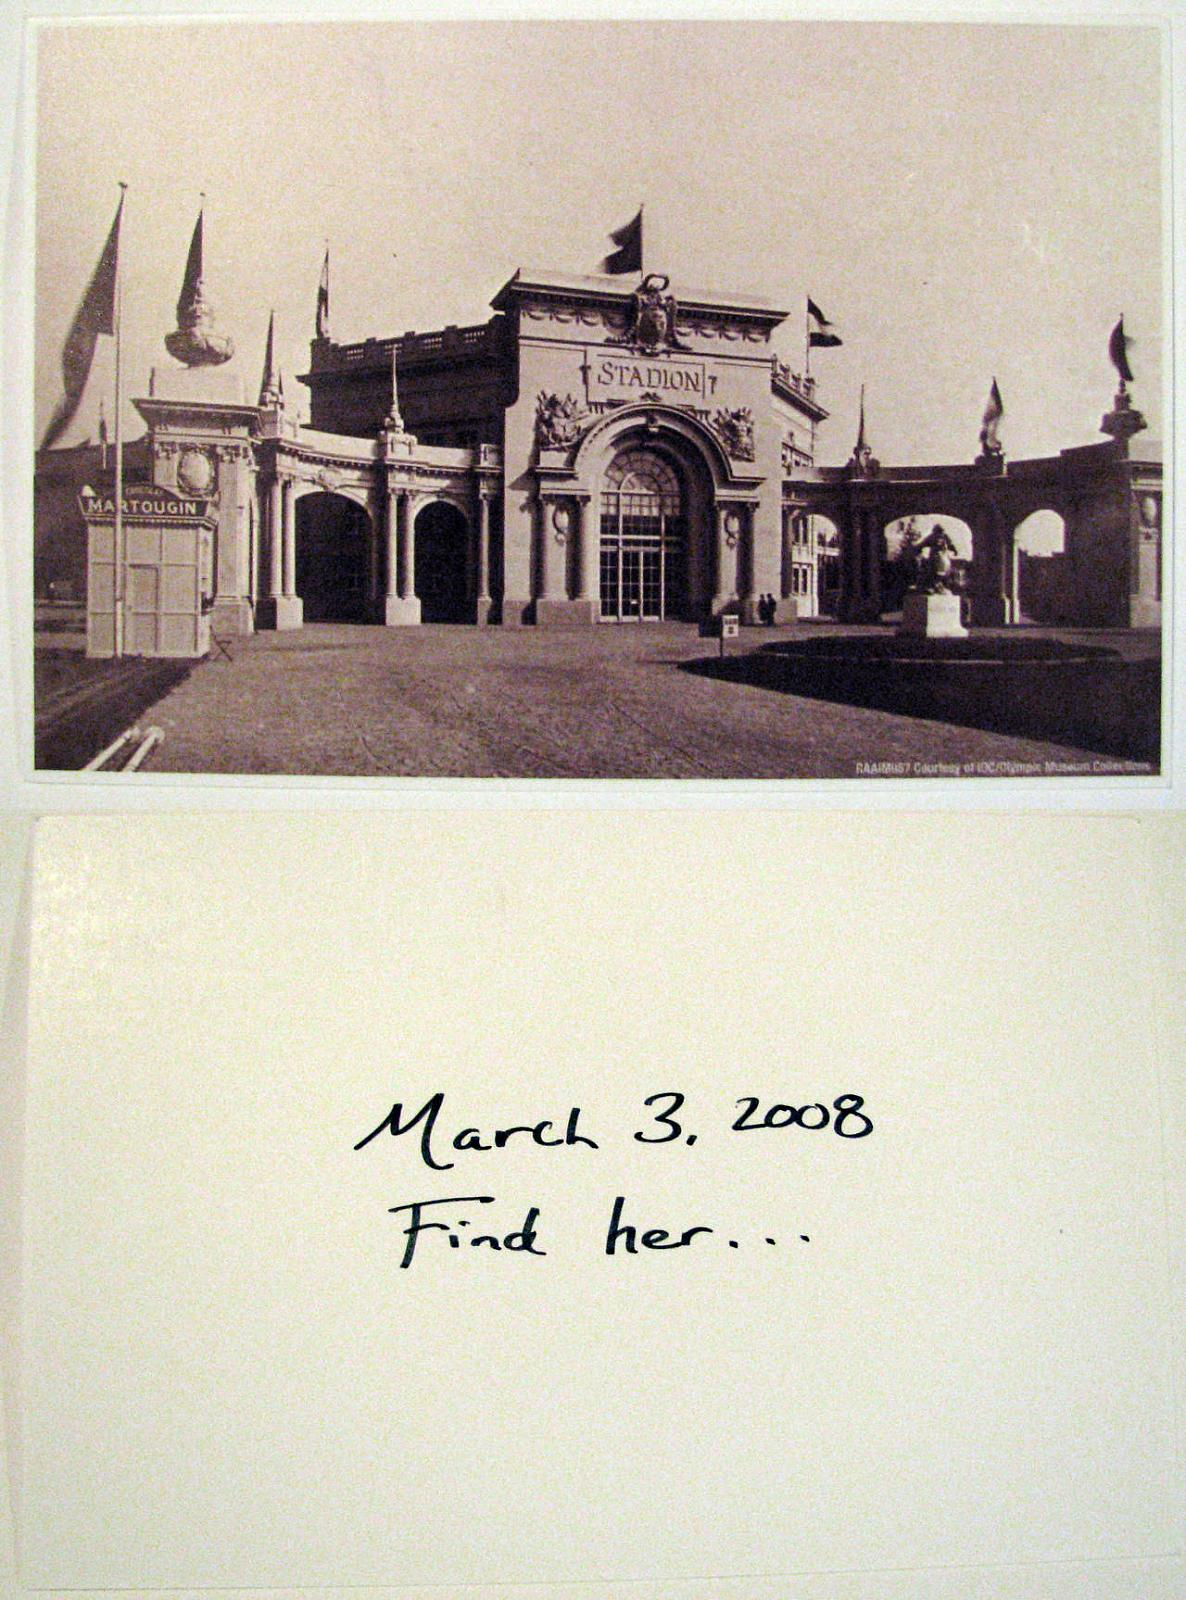
\includegraphics[width=3.95cm]{img/argTheLostRing/2299370206_89505225a9_o.jpg}
		\end{column}
		\begin{column}[T]{4.05cm}
			%% \item[] Carte Postale 3
			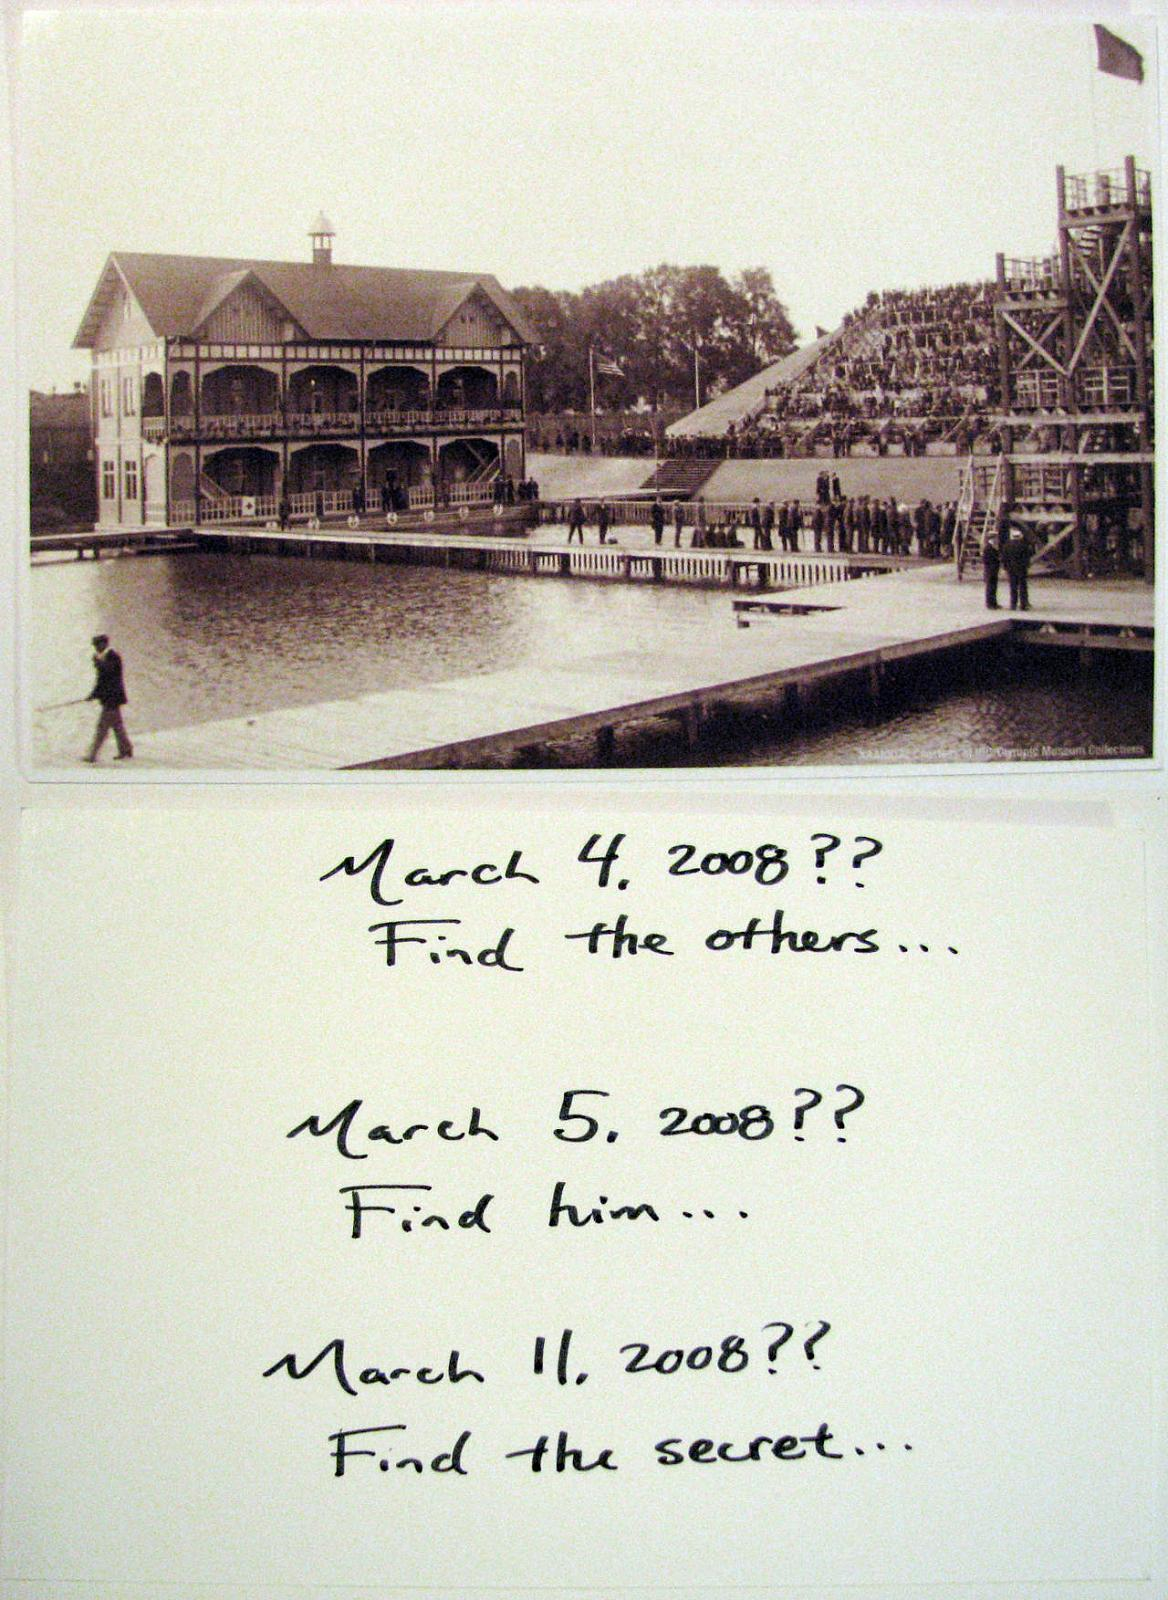
\includegraphics[width=3.95cm]{img/argTheLostRing/2298573497_9faf88fc1d_o.jpg}
		\end{column}
	\end{columns}
\end{frame} 

% \begin{frame}
	% \frametitle{\moreInFrameTitleLeftt \sectionPartIIaIV  (4) }
	% \begin{itemize}
		% \item Carte Postale 1 recto / Verso...
		% 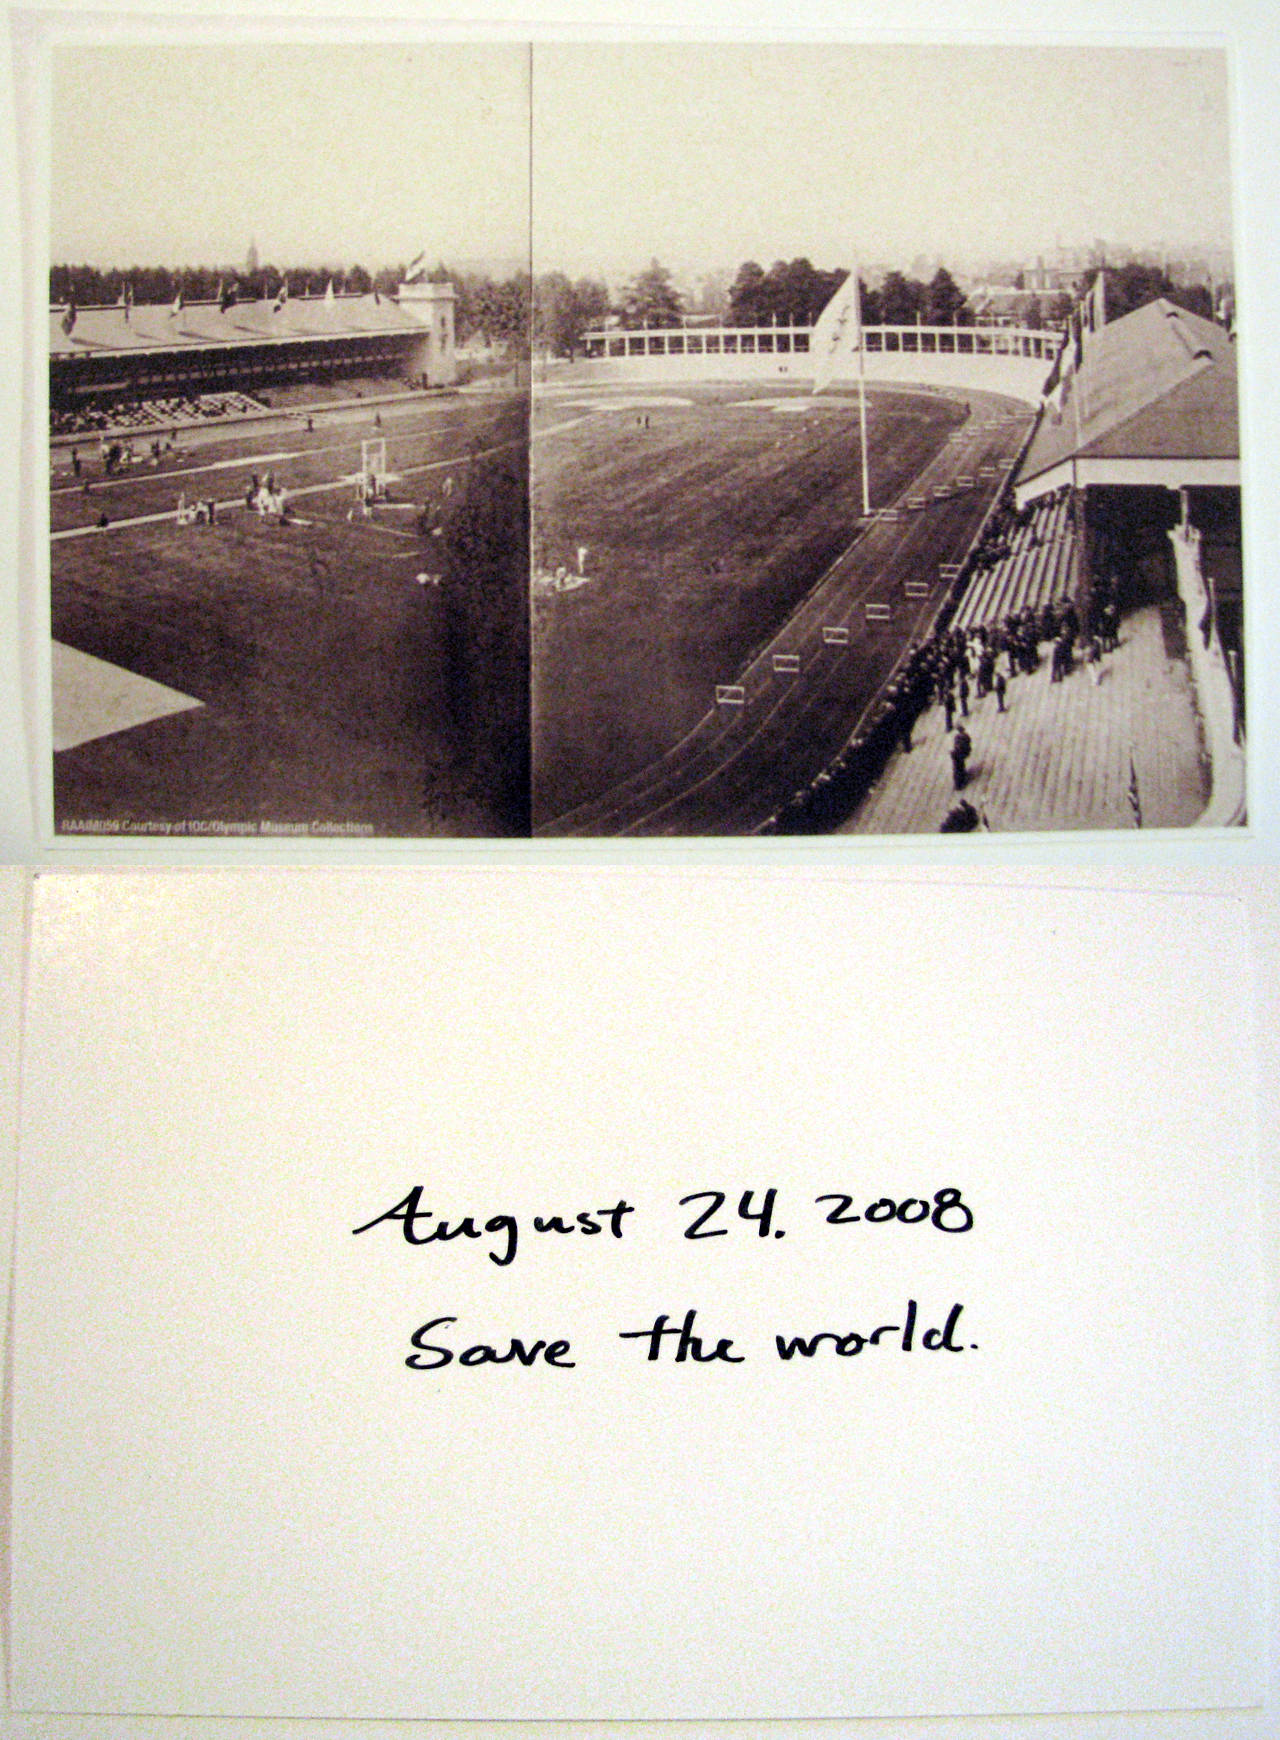
\includegraphics[height=7.00cm]{img/argTheLostRing/2299369980_6cd3e50860_o.jpg}
	% \end{itemize}
% \end{frame} 

% \begin{frame}
	% \frametitle{\moreInFrameTitleLeftt \sectionPartIIaIV  (5) }
	% \begin{itemize}
		% \item Carte Postale 2 recto / Verso...
		% 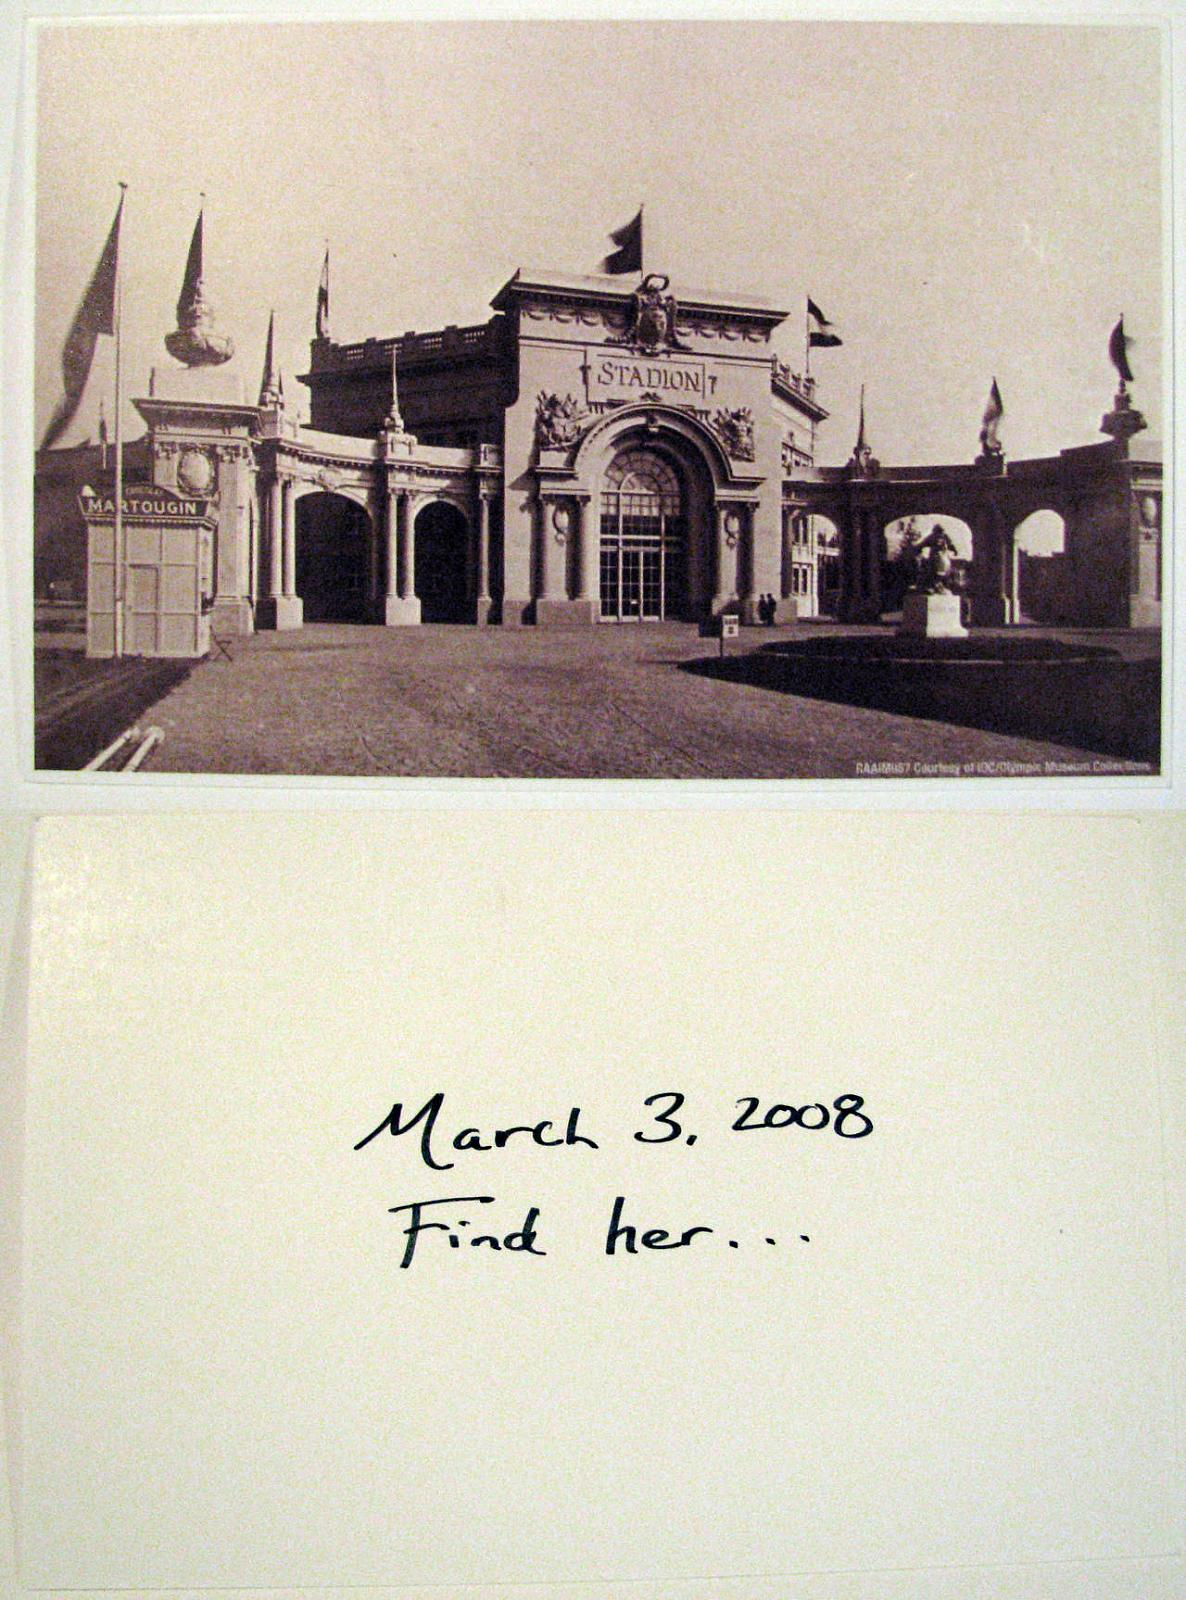
\includegraphics[height=7.00cm]{img/argTheLostRing/2299370206_89505225a9_o.jpg}
	% \end{itemize}
% \end{frame} 

% \begin{frame}
	% \frametitle{\moreInFrameTitleLeftt \sectionPartIIaIV  (6) }
	% \begin{itemize}
		% \item Carte Postale 3 recto / Verso...
		% 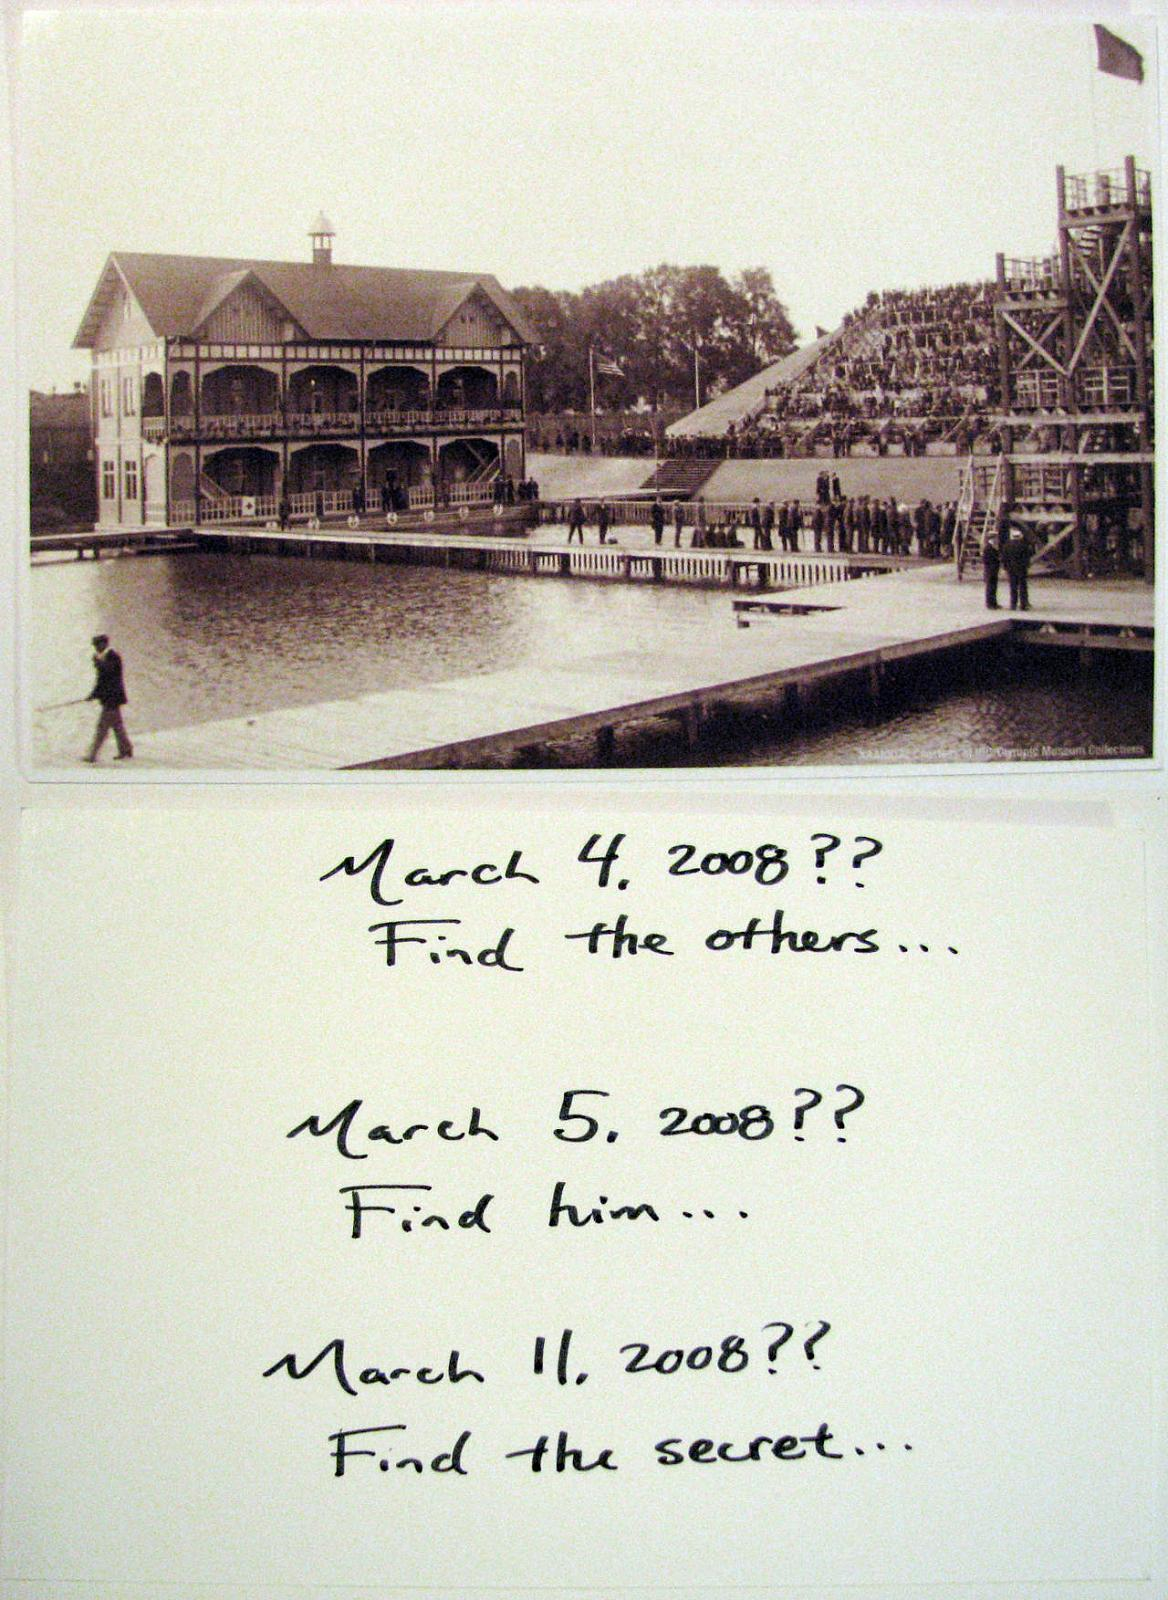
\includegraphics[height=7.00cm]{img/argTheLostRing/2298573497_9faf88fc1d_o.jpg}
	% \end{itemize}
% \end{frame} 

\begin{frame}
	\frametitle{\moreInFrameTitleLeftt \sectionPartIIaIV  (5) }
	\begin{itemize}
		\item Une pelote de laine / un fil d'Ariane ?
		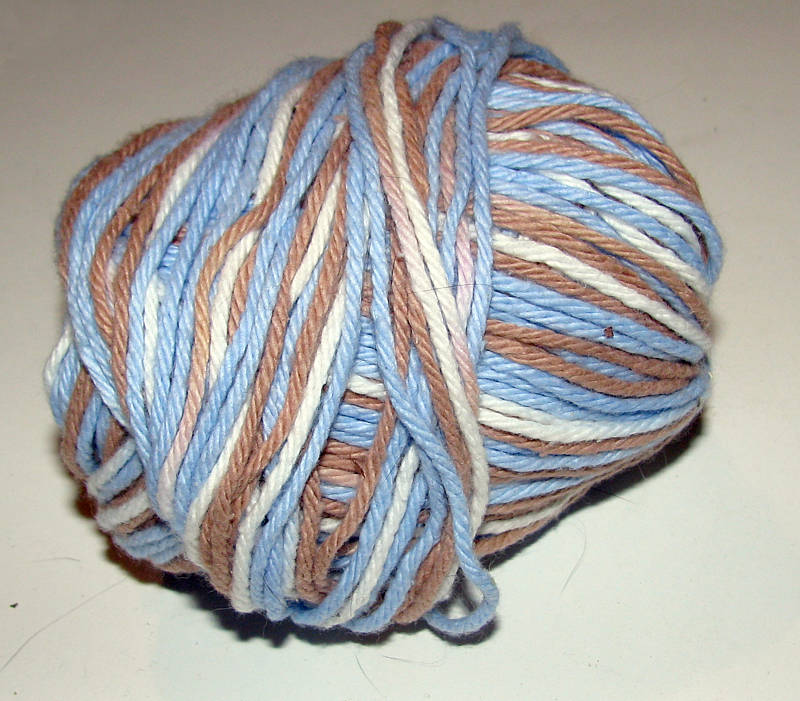
\includegraphics[height=7.00cm]{img/argTheLostRing/2299401072_b1ddc63acc_o.jpg}
	\end{itemize}
\end{frame}

\begin{frame}
	\frametitle{\moreInFrameTitleLeftt \sectionPartIIaIV  (6) }
	\begin{columns}[T]
		\begin{column}[T]{5.05cm}
			\begin{itemize}
				\item Boite FedEx + Affiche + cartes postales + pelote de laine => Promotion des Jeux Olympiques de 2008
				\item Jeux d'envergure mondiale (blog, biblioth{\`e}ques...) : recherche d'indices dans les principales villes du monde, 
				\item Rassemblement d'un codex {\'e}crit en... esperanto, d{\'e}crivant un "sport perdu" pour synchroniser des mondes parall{\`e}les !
			\end{itemize}
		\end{column}
		\begin{column}[T]{5.05cm}
			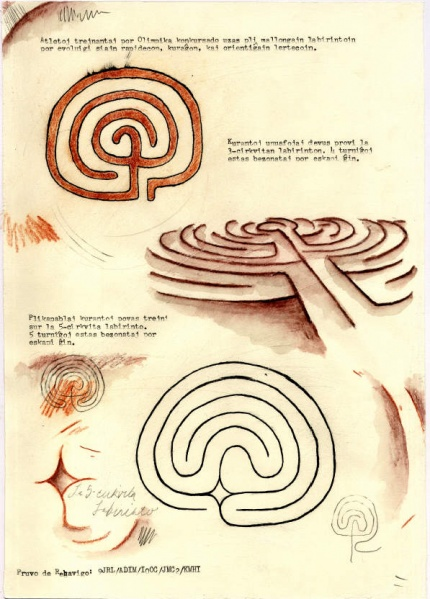
\includegraphics[width=5.00cm]{img/argTheLostRing/430px-CotLR-4Ap2.jpg}~\\
			\texttt{\footnotesize http://olympics.wikibruce.com/Home}
		\end{column}
	\end{columns}
\end{frame}

\def\sectionPartIIaV{Majestic}
\subsubsection{\sectionPartIIaV} %% TODO Majestic => insister sur aspect transmedia ?!
\begin{frame}
	\frametitle{\moreInFrameTitleLeftt \sectionPartIIaV  (1) }
	%% \begin{itemize}
	%% 	\item \textbf{ \sectionPartIIaV }
	%% \end{itemize}
	
	\begin{columns}[T]
		\begin{column}[T]{5.05cm}
			
\includegraphics[width=5.00cm]{img/majesticARGgame/majestic-screenshot-ME0000034566_2.jpg}~\\
			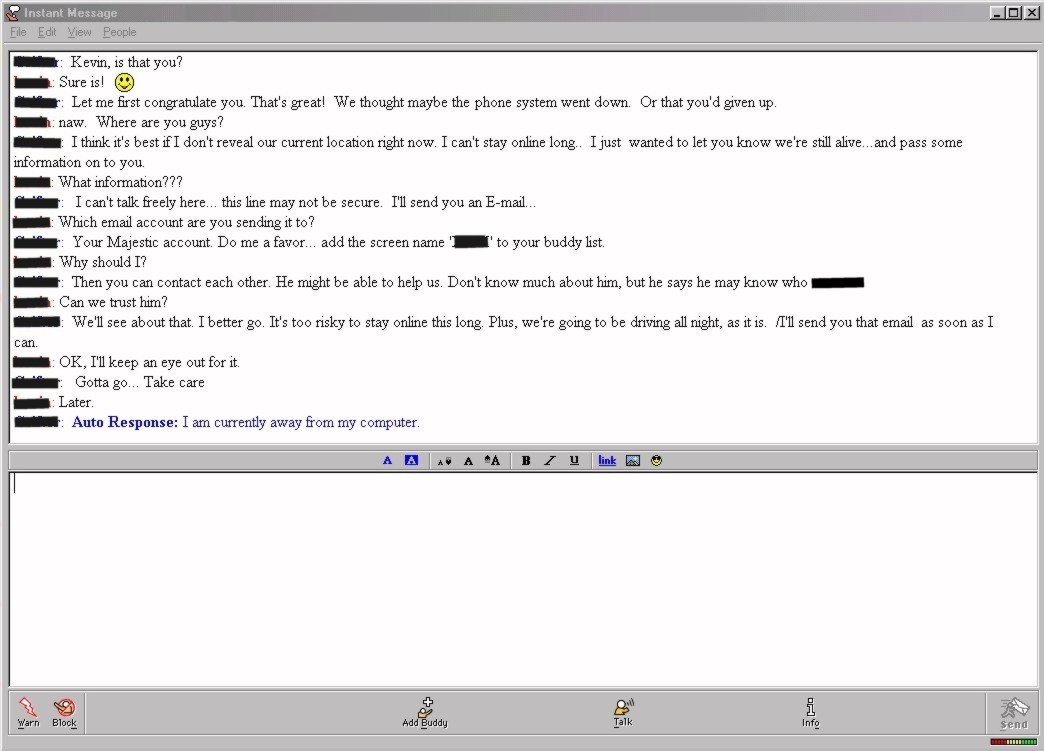
\includegraphics[width=5.00cm]{img/majesticARGgame/ca-a-bien-change-teens-irc-net-ME0000034567_2.jpg}~\\
		\end{column}
		\begin{column}[T]{5.05cm}
			\begin{itemize}
				\item Jeu vid{\'e}o bas{\'e} sur des th{\'e}ories de la conspiration gouvernementales, 
				\item Aspects \emph{transmedia} et temps r{\'e}el : t{\'e}l{\'e}phone, courriel, Messagerie instantan{\'e}e, Fax, Sites Web...
				\item Rattrap{\'e} par l'actualit{\'e} r{\'e}elle : sorti le 31 juillet 2001, mis en pause le 11 septembre 2001, 
				\item N'a jamais retrouv{\'e} de succ{\`e}s malgr{\'e} des prix d'innovation. 
			\end{itemize}
		\end{column}
	\end{columns}
\end{frame} 

\begin{frame}
	\frametitle{\moreInFrameTitleLeftt \sectionPartIIaV  (2) }
	\begin{columns}[T]
		\begin{column}[T]{5.05cm}
			
\includegraphics[width=5.00cm]{img/majesticARGgame/majestic-screenshot-ME0000046986_2.jpg}~\\
			\texttt{\footnotesize L'interface principale }
		\end{column}
		\begin{column}[T]{5.05cm}
			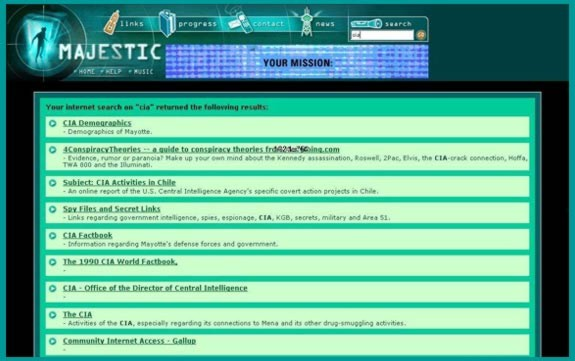
\includegraphics[width=5.00cm]{img/majesticARGgame/majestic-screenshot-ME0000046985_2.jpg}~\\
			\texttt{\footnotesize "Votre mission" et recherches }
		\end{column}
	\end{columns}
\end{frame}

\begin{frame}
	\frametitle{\moreInFrameTitleLeftt \sectionPartIIaV  (3) }
	\begin{columns}[T]
		\begin{column}[T]{5.05cm}
			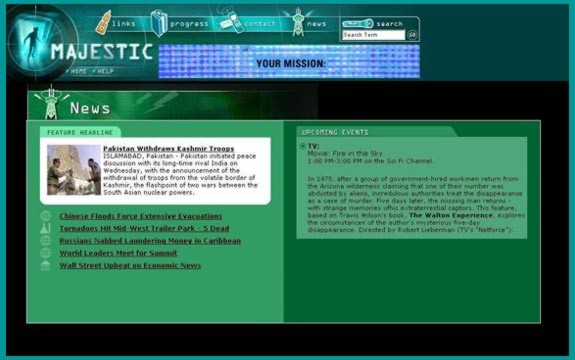
\includegraphics[width=5.00cm]{img/majesticARGgame/majestic-screenshot-ME0000046987_2.jpg}~\\
			\texttt{\footnotesize "Votre mission", {\'e}v{\`e}nements, nouvelles... }
		\end{column}
		\begin{column}[T]{5.05cm}
			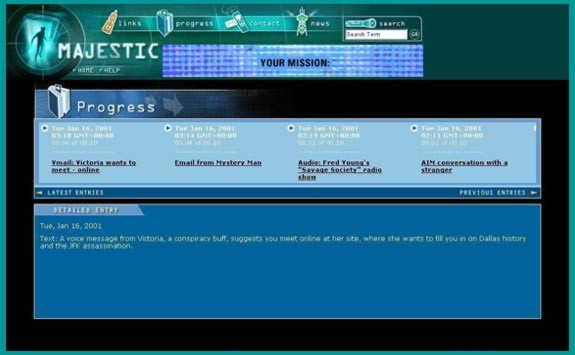
\includegraphics[width=5.00cm]{img/majesticARGgame/majestic-screenshot-ME0000046990_2.jpg}~\\
			\texttt{\footnotesize "Votre mission" : progression }
		\end{column}
	\end{columns}
\end{frame}

\begin{frame}
	\frametitle{\moreInFrameTitleLeftt \sectionPartIIaV  (4) }
	\begin{columns}[T]
		\begin{column}[T]{5.05cm}
			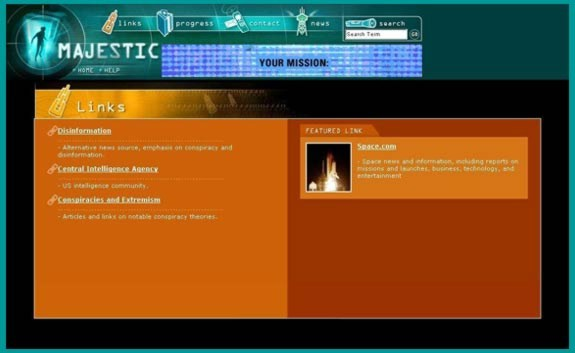
\includegraphics[width=5.00cm]{img/majesticARGgame/majestic-screenshot-ME0000046991_2.jpg}~\\
			\texttt{\footnotesize "Votre mission" : liens (dans le jeu et hors jeu) }
		\end{column}
		\begin{column}[T]{5.05cm}
			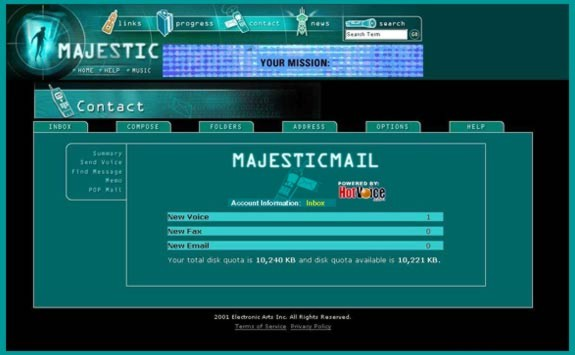
\includegraphics[width=5.00cm]{img/majesticARGgame/majestic-screenshot-ME0000046992_2.jpg}~\\
			\texttt{\footnotesize "Votre mission" : interface de courriels d{\'e}di{\'e}e }
		\end{column}
	\end{columns}
\end{frame}

\begin{frame}
	\frametitle{\moreInFrameTitleLeftt \sectionPartIIaV  (5) }
	\begin{columns}[T]
		\begin{column}[T]{5.05cm}
			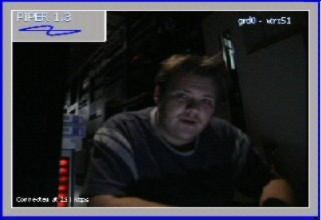
\includegraphics[width=5.00cm]{img/majesticARGgame/tu-fais-ch-joe-tu-sais-quelle-heure-il-est-ici-ME0000034570_2.jpg}~\\
			\texttt{\footnotesize Vid{\'e}oconf{\'e}rences... }
		\end{column}
		\begin{column}[T]{5.05cm}
			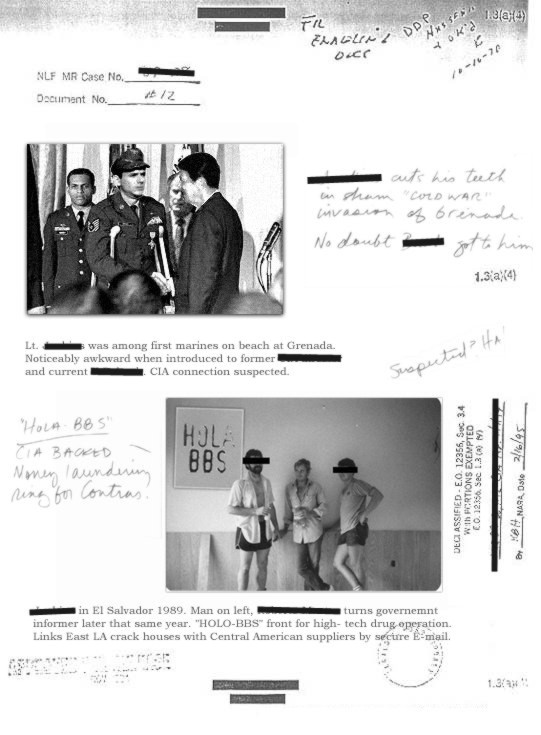
\includegraphics[width=5.00cm]{img/majesticARGgame/youve-got-fax-ME0000034568_2.jpg}~\\
		\end{column}
	\end{columns}
\end{frame}

\def\sectionPartIIaVI{ This is Not a Game (WJW) }
\subsubsection{\sectionPartIIaVI}
\begin{frame}
	\frametitle{\moreInFrameTitleLeftt \sectionPartIIaVI }
	%% \begin{itemize}
	%% 	\item \textbf{ \sectionPartIIaVI }
	%% \end{itemize}
	\begin{columns}[T]
		\begin{column}[T]{4.1cm}
			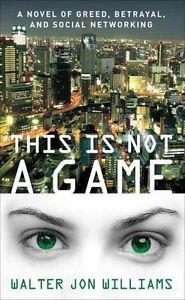
\includegraphics[height=4.05cm]{img/thisIsNotAGameWJW.jpg}
		\end{column}
		\begin{column}[T]{7cm}
			 \begin{beamerboxesrounded}	[lower=substructureRED, %
							 upper=block title RED,%
							 shadow=true]%
				   {\sectionPartIIaVI}
				\begin{itemize}
					\item \emph{This Is Not A Game} (Walter Jon Williams)
					\item Fiction contemporaine
					\item {\`A} la fois dans le jeu et hors jeu
					\item En Fran\c{c}ais : \emph{Ceci n'est pas un jeu}
					\item ...
				\end{itemize}
			\end{beamerboxesrounded}
		\end{column}
	\end{columns}
\end{frame} 

\def\sectionPartIIaVII{The Web Soap}
\subsubsection{\sectionPartIIaVII}
\begin{frame}
	\frametitle{\moreInFrameTitleLeftt \sectionPartIIaVII }
	%% \begin{itemize}
	%% 	\item \textbf{ \sectionPartIIaVII }
	%% \end{itemize}
	\begin{columns}[T]
		\begin{column}[T]{5.00cm}
			\begin{itemize}
				\item \emph{Proto-}ARG
				\item Fiction contemporaine
				\item \emph{Le Web Soap, un conte disloqu{\'e}} (transfert.net 24/09/2000)
				\item "Douze auteurs et douze personnages"
				\item "Une histoire sans fin"
			\end{itemize}
		\end{column}
		\begin{column}[T]{5.00cm}
			\begin{itemize}
				\item Organis{\'e} en {\'e}pisodes
				\item Sites Web ET Blogs ET rencontres IRL
				\item ...
				\item Archives du site \emph{transfert.net}
				\item ...
				%% \item \texttt{http://www.transfert.net/Le-Web-Soap-un-conte-disloque}
				%% \item \texttt{http://www.transfert.net/ARCHIVES-1-09-Le-Web-reinvente-le}
			\end{itemize}
		\end{column}
	\end{columns}
\end{frame} 


\def\sectionPartIIaVIII{Resistance Radio}
\subsubsection{\sectionPartIIaVIII}
\begin{frame}
	\frametitle{\moreInFrameTitleLeftt \sectionPartIIaVIII  (1) }
	\begin{columns}[T]
		\begin{column}[T]{5.05cm}
			\begin{itemize}
				%% \item \textbf{ \sectionPartIIaVIII }
				\item En compl{\'e}ment de la s{\'e}rie T{\'e}l{\'e}vis{\'e}e \emph{The Man In the High Castle}, 
				\item Une radio {\'e}met depuis la zone neutre,  
				\item Fait partie de l'ambiance immersive...
			\end{itemize}
			
			
\includegraphics[width=3.00cm]{img/ResistanceRadio/resistance-radio-700x401.jpg}~\\
			
		\end{column}
		\begin{column}[T]{5.05cm}
			
\includegraphics[width=5.00cm]{img/ResistanceRadio/USA_in_The_Man_in_the_High_Castle-640x377}~\\
			\texttt{L'Am{\'e}rique du Nord dans les ann{\'e}es 1960 alternatives...}
		\end{column}
	\end{columns}
\end{frame} 

\begin{frame}
	\frametitle{\moreInFrameTitleLeftt \sectionPartIIaVIII  (2) }
	\begin{columns}[T]
		\begin{column}[T]{5.05cm}
			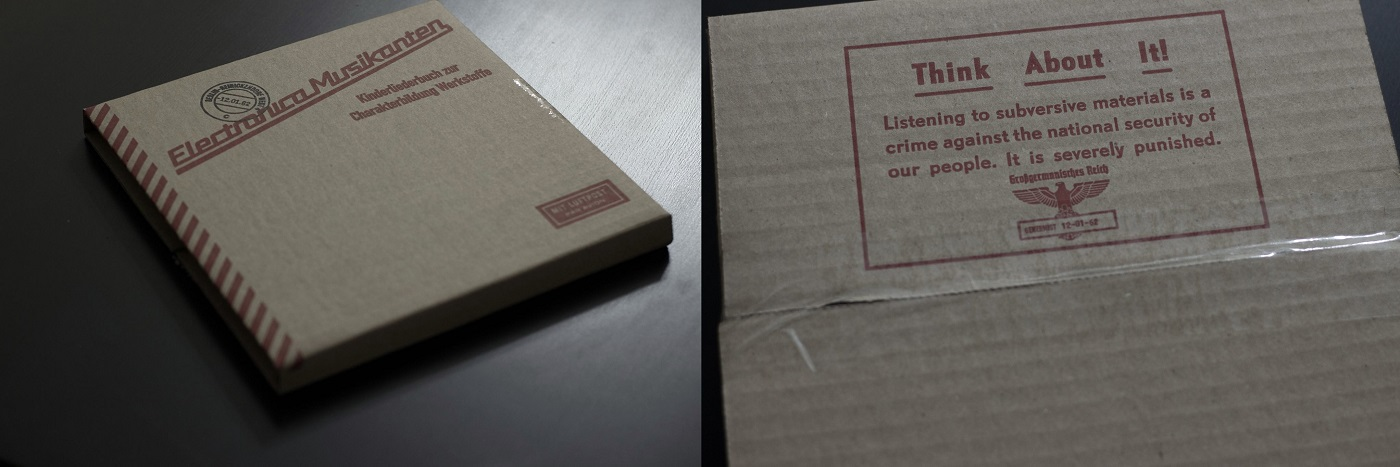
\includegraphics[width=5.00cm]{img/ResistanceRadio/electronica-musikanten.jpg}~\\
			~\\
			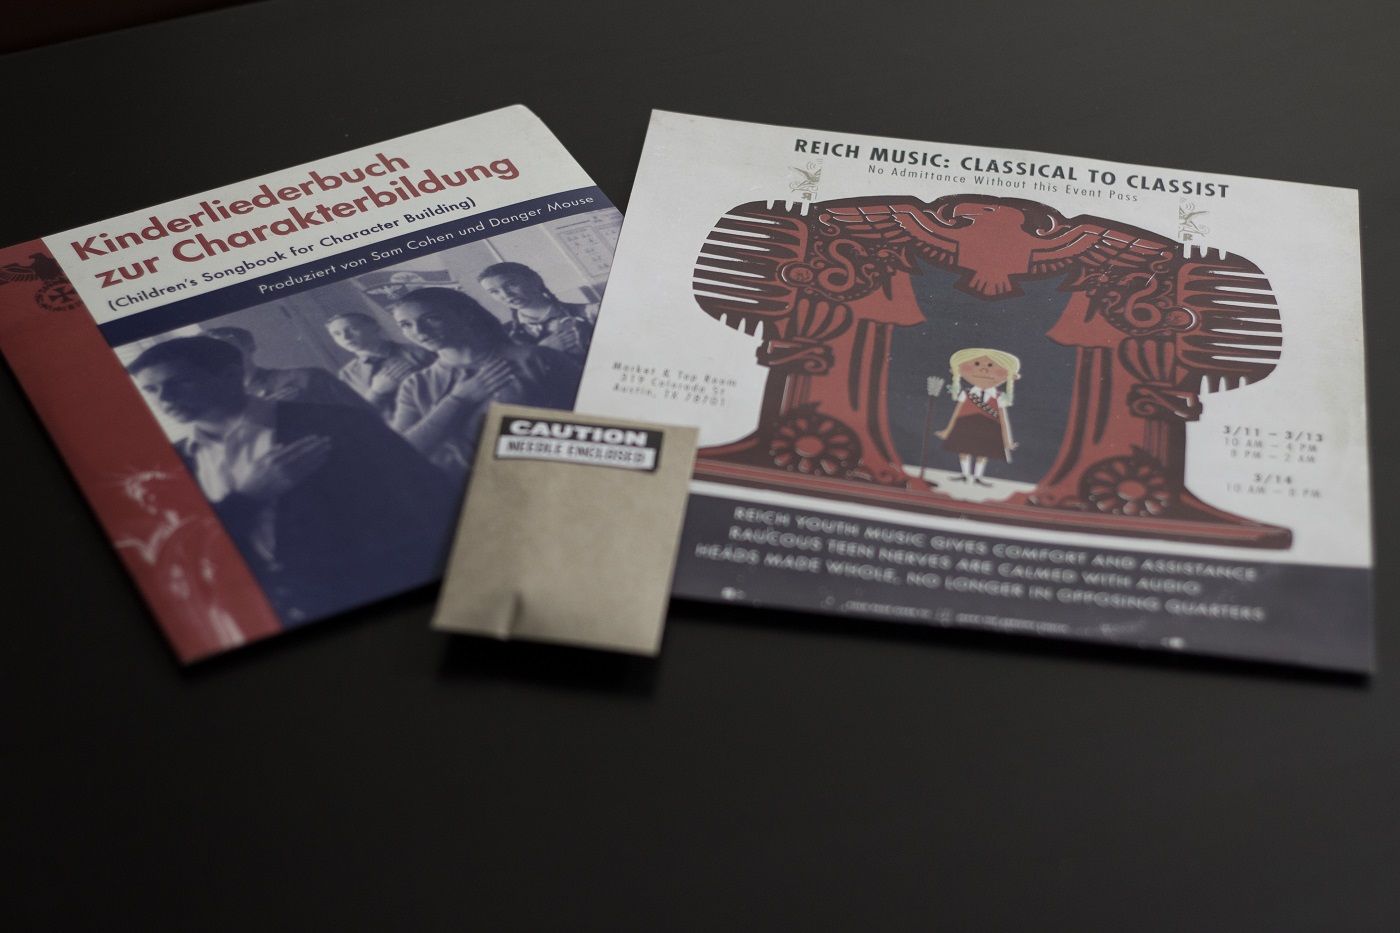
\includegraphics[width=5.00cm]{img/ResistanceRadio/resistance-radio-reich-small.jpg}~\\
		\end{column}
		\begin{column}[T]{5.05cm}
			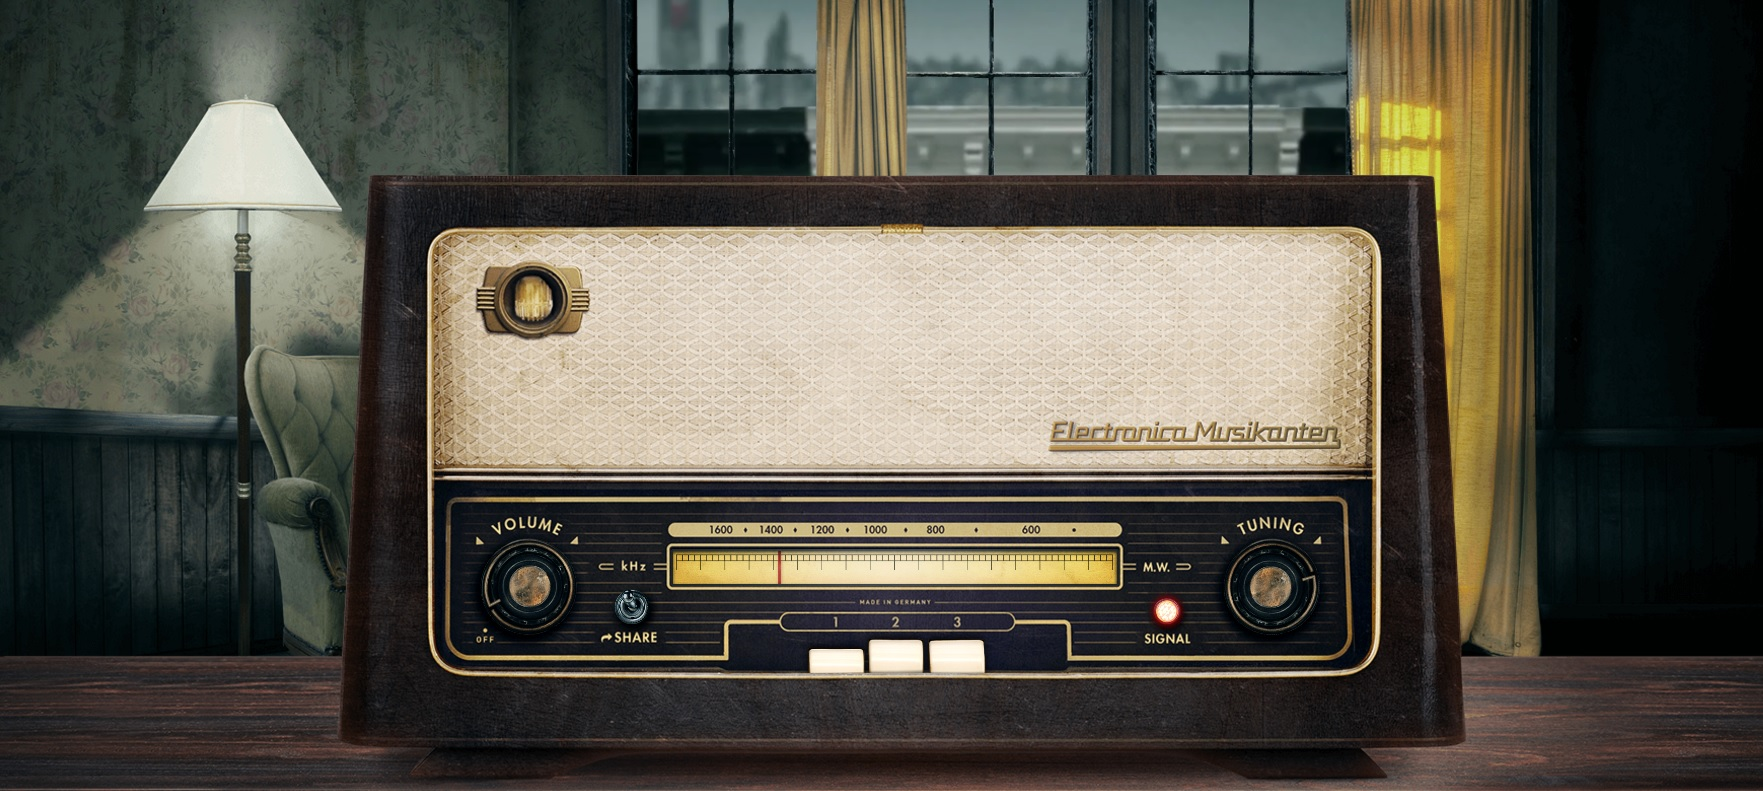
\includegraphics[width=5.00cm]{img/ResistanceRadio/resistance-radio-image.jpg}~\\
			
			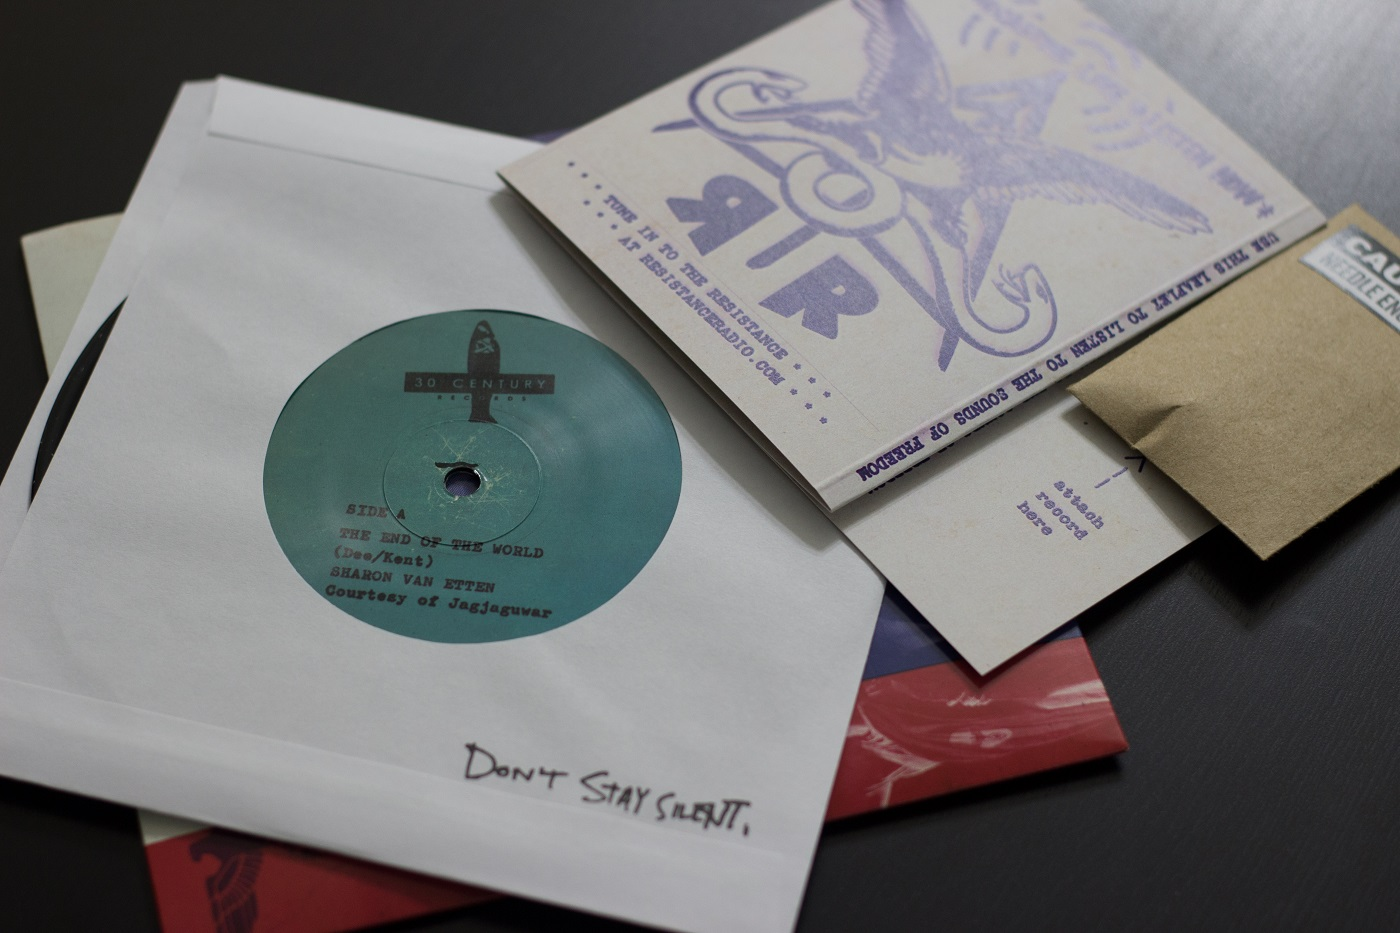
\includegraphics[width=5.00cm]{img/ResistanceRadio/resistance-radio-secret-contents-small.jpg}~\\
		\end{column}
	\end{columns}
\end{frame}

\begin{frame}
	\frametitle{\moreInFrameTitleLeftt \sectionPartIIaVIII  (3) }
	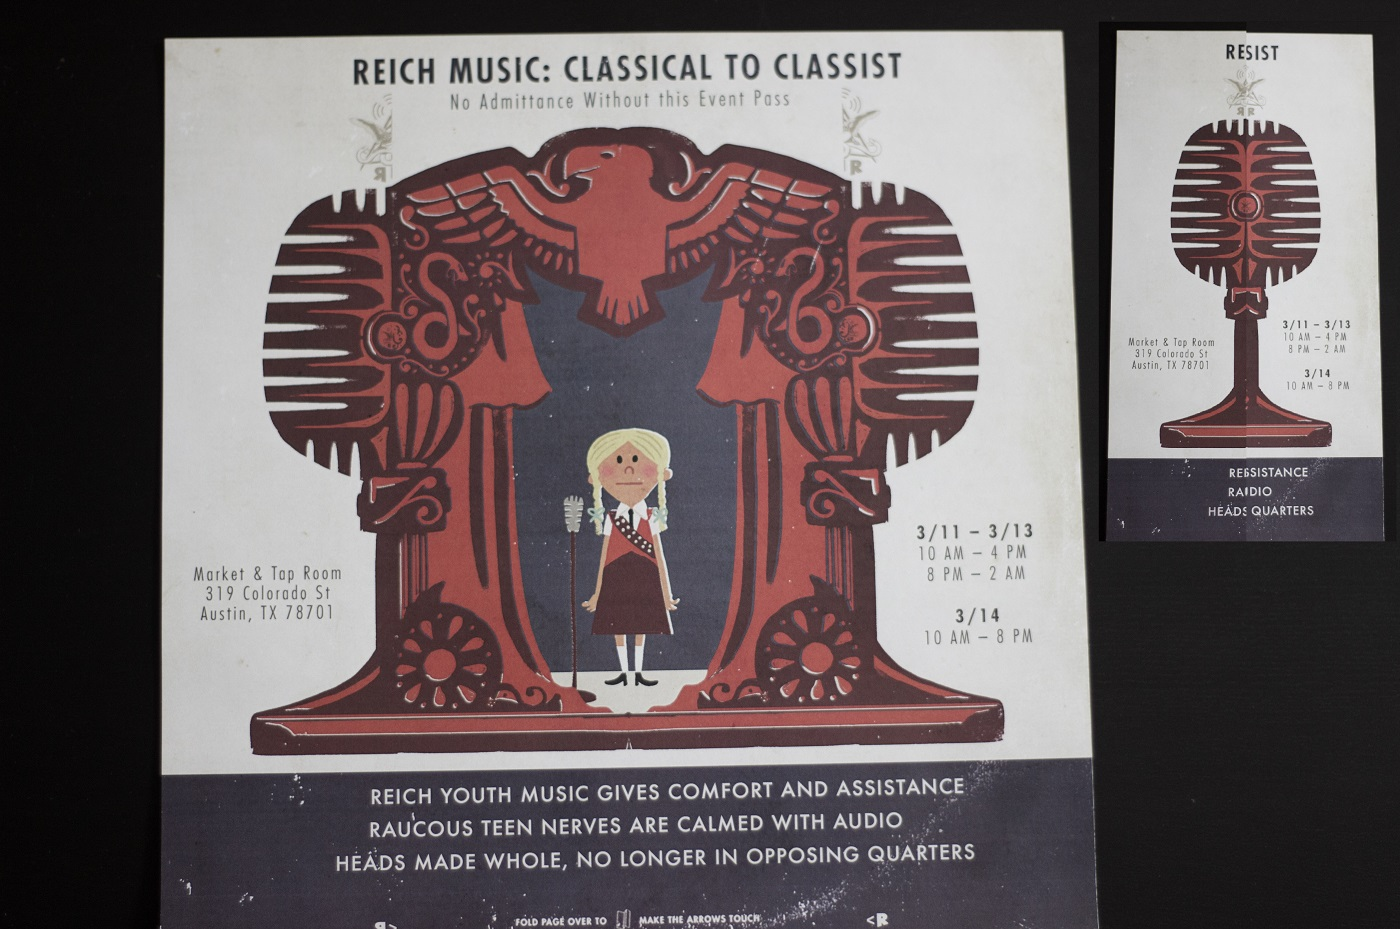
\includegraphics[width=10.00cm]{img/ResistanceRadio/resistance-radio-secret-solved.jpg}~\\
\end{frame}



\def\sectionPartIIb{Principes g{\'e}n{\'e}raux}
\subsection{\sectionPartIIb} %% Principes G{\'e}n{\'e}raux
\begin{frame}
	\frametitle{\moreInFrameTitleLeftt \sectionPartIIb }
	\tableofcontents[sections=2,currentsection,subsectionstyle=show/shaded/hide]
\end{frame} 

\def\sectionPartIIbI{Transmedia : InterNet, InterWeb (et le reste)}
\subsubsection{\sectionPartIIbI} %% Transmedia
\begin{frame}
	\frametitle{\moreInFrameTitleLeftt \sectionPartIIbI }
	\begin{itemize}
		\item \textbf{ \sectionPartIIbI }
		\begin{itemize}
			\item Sites web, Courrier {\'E}lectronique, canaux IRC, forums, messageries instantan{\'e}es... ; 
			\item r{\'e}seaux sociaux (FaceBook, Twitter...) ; 
			\item SMS, appels t{\'e}l{\'e}phoniques... ; 
			\item Courrier postal, articles de journaux, petites annonces...
			\item T{\'e}l{\'e}vision / Cin{\'e}ma, Street Art, encarts publicitaires...
		\end{itemize}
		\item M{\'e}lange r{\'e}el et fictionnel via le virtuel !
	\end{itemize}
\end{frame} 

\def\sectionPartIIbII{Chasse aux tr{\'e}sors (et {\'e}nigmes)}
\subsubsection{\sectionPartIIbII} %% Chasse aux tr{\'e}sors & {\'e}nigmes
\begin{frame}
	\frametitle{\moreInFrameTitleLeftt \sectionPartIIbII }
	\begin{itemize}
		\item \textbf{ \sectionPartIIbII }
		\item[] ...
		\item \textcolor{red}{ \textbf{TODO} }
	\end{itemize}
\end{frame} 

\def\sectionPartIIbIII{La curiosit{\'e} (et le reste) : deux groupes}
\subsubsection{\sectionPartIIbIII} %% Deux groupes
\begin{frame}
	\frametitle{\moreInFrameTitleLeftt \sectionPartIIbIII }
	%% \begin{itemize}
	%% 	\item \textbf{ \sectionPartIIbIII }
	%% \end{itemize}
	\begin{columns}[T]
		\begin{column}[T]{5.10cm}
			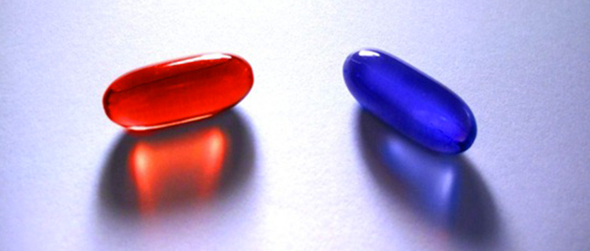
\includegraphics[width=5.05cm]{img/ob_0ce702_pillules.jpg}~\\
			%% \texttt{\footnotesize Rouge : le Virtuel, Bleu : le R{\'e}el ; ARG / JRA : un m{\'e}lange des deux ? }~\\
			\texttt{\footnotesize Rouge : le Monde R{\'e}el du Quotidien, Bleu : l'Univers Fictif du Jeu ; ARG / JRA : un m{\'e}lange des deux ?! }~\\
			\texttt{ http://www.metacortechs.com/ }
		\end{column}
		\begin{column}[T]{5.80cm}
			 \begin{beamerboxesrounded}	[lower=substructureRED, %
							 upper=block title RED,%
							 shadow=true]%
				   {\sectionPartIIbIII}
				\begin{itemize}
					\item Toujours au moins deux publics (exemple de \emph{The Lost Experience})
					\item 1/ Un public d'ensemble, qui ne verra m{\^e}me pas le jeu / les {\'e}nigmes, 
					\item 2/ Un public de curieux, qui suivra les accroches et {\'e}nigmes
					\item ...
					\item \emph{Quel est le public cible ?}
				\end{itemize}
			\end{beamerboxesrounded}
		\end{column}
	\end{columns}
\end{frame} 

\def\sectionPartIIbIV{{\'E}vidences et formats / tailles : audiences}
\subsubsection{\sectionPartIIbIV} %% Audiences
\begin{frame}
	\frametitle{\moreInFrameTitleLeftt \sectionPartIIbIV }
	\begin{itemize}
		\item \textbf{ \sectionPartIIbIV }
		\item[] ...
		\item \textcolor{red}{ \textbf{TODO} }
	\end{itemize}
\end{frame} 

\def\sectionPartIIbV{Communaut{\'e}s}
\subsubsection{\sectionPartIIbV} %% Communaut{\'e}s
\begin{frame}
	\frametitle{\moreInFrameTitleLeftt \sectionPartIIbV }
	\begin{itemize}
		\item \textbf{ \sectionPartIIbV }
		\item[] ...
		\item \textcolor{red}{ \textbf{TODO} }
	\end{itemize}
\end{frame} 


\def\sectionPartIIc{Id{\'e}es et compl{\'e}ments}
\subsection{\sectionPartIIc} %% Id{\'e}es et compl{\'e}ments
\begin{frame}
	\frametitle{\moreInFrameTitleLeftt \sectionPartIIc }
	\tableofcontents[sections=2,currentsection,subsectionstyle=show/shaded/hide]
\end{frame} 

\def\sectionPartIIcI{Pourquoi faire un ARG ?}
\subsubsection{\sectionPartIIcI} %% Pourquoi un ARG ?
\begin{frame}
	\frametitle{\moreInFrameTitleLeftt \sectionPartIIcI }
	\begin{itemize}
		\item Promouvoir un {\'e}v{\`e}nement (exemple des Jeux Olympiques 2008 avec \emph{The Lost Ring}), 
		\item Promouvoir un {\'e}l{\'e}ment commercial ponctuel (film, jeu vid{\'e}o...) qui auto-alimente le jeu ?! (les exemples sont l{\'e}gions), 
		\item Loisir / culture / tourisme (visite d'un mus{\'e}e par exemple ou d'un lieu d'int{\'e}r{\^e}t) (ex : \emph{Can You Stop It ?} pour \emph{Lille 3000 / Europe XXL} en 2009), 
		\item[] ...
		\item Des id{\'e}es ?
	\end{itemize}
\end{frame} 

\def\sectionPartIIcII{Parall{\`e}le avec le JdR / Jeu de R{\^o}le}
\subsubsection{\sectionPartIIcII} %% Parall{\`e}le avec le JdR
\begin{frame}
	\frametitle{\moreInFrameTitleLeftt \sectionPartIIcII }
	\begin{itemize}
		\item Sc{\'e}nario, 
		\item Meneur de Jeu (plut{\^o}t \emph{PuppetMaster} ou Marionnettiste dans le cas des ARG), 
		\item Aspect "m{\'e}ta-jeu" et immersion dans le r{\'e}el, notion de TINAG / \emph{This Is Not A Game}, 
		\item Le rideau / \emph{The Curtain} : la diff{\'e}rentiation avec le re{\'e}l (parfois notion de "quatri{\`e}me mur"), 
		\item Le terrier du lapin / \emph{The Rabbit Hole} : la (ou les) accroche(s) initiale(s) du sc{\'e}nario. 
	\end{itemize}
\end{frame} 

\def\sectionPartIIcIII{Parall{\`e}le avec le Jeu Vid{\'e}o}
\subsubsection{\sectionPartIIcIII} %% Parall{\`e}le avec le Jeu Vid{\'e}o (+ MMORPG ?!)
\begin{frame}
	\frametitle{\moreInFrameTitleLeftt \sectionPartIIcIII }
	\begin{itemize}
		\item Implication de groupe autour d'une ou de plusieurs "qu{\^e}tes" ; 
		\item Travail seul / en {\'e}quipe (comp{\'e}tences compl{\'e}mentaires) ; 
		\item Mise en commun des informations. 
	\end{itemize}
\end{frame} 

% ***************************************
% ******     III <<Pack Bonus>>   *******
% ***************************************

\def\sectionPartIII{Id{\'e}es analogues : (re)d{\'e}couvrir le monde}
\section{\sectionPartIII}
\begin{frame}
	\frametitle{\moreInFrameTitleLeftt \sectionPartIII}
	\tableofcontents[sections=3,currentsection,subsectionstyle=show/shaded/hide] %% ,sectionstyle=hide/hide
\end{frame} 

% \subsection{\sectionPartIII}
% \begin{frame}
	% \frametitle{\moreInFrameTitleLeftt \sectionPartIII}
	% \tableofcontents[sections=3,currentsection,subsectionstyle=show/shaded/hide]
% \end{frame} 

\def\sectionPartIIIa{"17 avril 1967 : ici il ne s'est rien pass{\'e}"}
\subsection{\sectionPartIIIa}
\begin{frame}
	\frametitle{\moreInFrameTitleLeftt \sectionPartIIIa}
	\begin{center}
		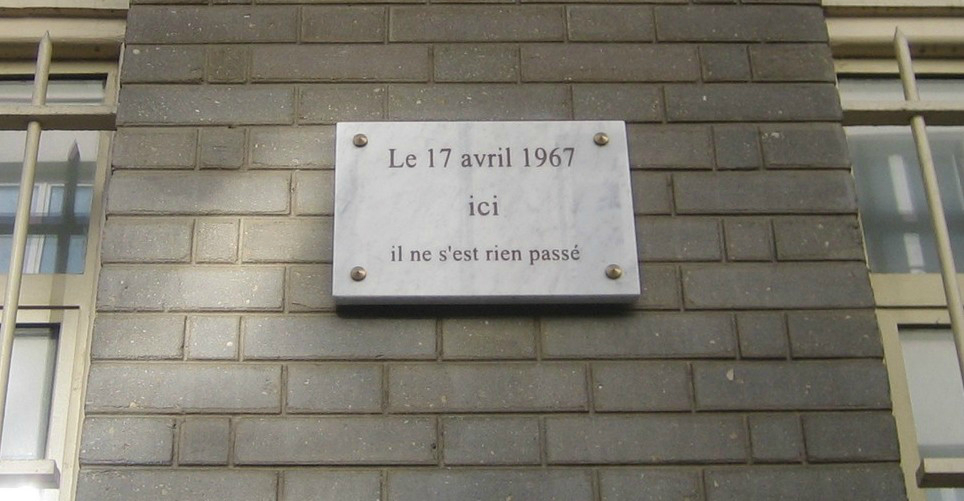
\includegraphics[height=6.5cm,width=11.0cm]{img/84869389_o.png} ~\\ %% [height=6.5cm,width=11.6cm]
		\texttt{\footnotesize Fausse plaque comm{\'e}moratives (appos{\'e}e en 2001-2002 {\`a} Paris)}
	\end{center}
\end{frame}

\def\sectionPartIIIb{"Street Wars", irruption dans le r{\'e}el}
\subsection{\sectionPartIIIb}
\begin{frame}
	\frametitle{\moreInFrameTitleLeftt \sectionPartIIIb}
	\begin{center}
		<<Tueurs {\`a} gages et pistolets {\`a} eau>>~\\
		(en France, {\`a} Paris et alentours, depuis 2007)
		%% 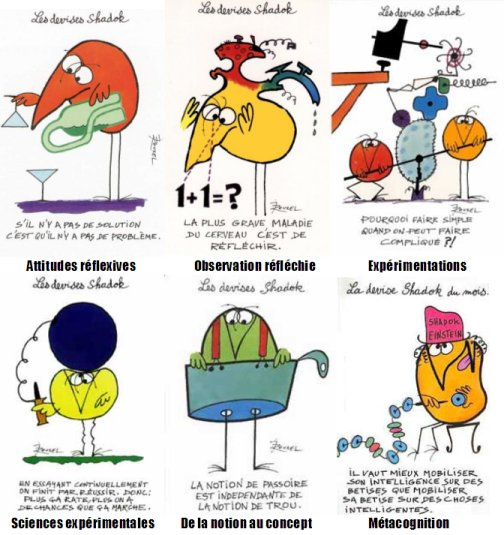
\includegraphics[height=6.5cm,width=11.6cm]{img/shadoks_devises.png} 
	\end{center}
\end{frame}

\def\sectionPartIIIc{"Vous avez vu les {\'e}nigmes dans cette pr{\'e}sentation ?"}
\subsection{\sectionPartIIIc}
\begin{frame}
	\frametitle{\moreInFrameTitleLeftt \sectionPartIIIc}
	\begin{center}
		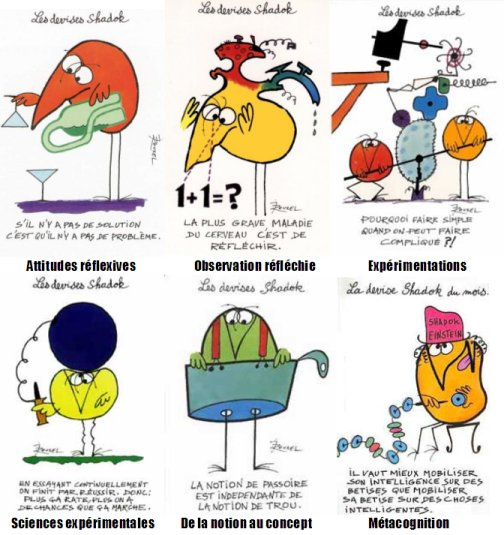
\includegraphics[height=7.0cm]{img/shadoks_devises.png} %% [height=6.5cm,width=11.6cm]
	\end{center}
\end{frame}

% \def\sectionPartIIId{"D{\'e}bats et controverses"}
% \subsection{\sectionPartIIId}
% \begin{frame}
	% \frametitle{\moreInFrameTitleLeftt \sectionPartIIId}
	% \begin{itemize}
		% \item Univers du divertissement : rattach{\'e} au jeu vid{\'e}o ?! Jeu de R{\^o}le Grandeur Nature (GN) ?
		% \item Effets sur le comportement du joueur (comme dans le jeu vid{\'e}o et d'autres jeux immersifs ;-) ), confusion r{\'e}el / fiction, virtuel, simulation. 
		% \item[] ...
	% \end{itemize}
% \end{frame}

\def\sectionPartIIIe{"D{\'e}bats et controverses" / "Cicada 3301", un ARG ?}
\subsection{\sectionPartIIIe}
\begin{frame}
	\frametitle{\moreInFrameTitleLeftt \sectionPartIIIe}
	\begin{columns}[T]
		\begin{column}[T]{5.05cm}
			\begin{itemize}
				\scriptsize 
				\item Univers du divertissement : rattach{\'e} au jeu vid{\'e}o ?! Jeu de R{\^o}le Grandeur Nature (GN) ?
				\item Effets sur le comportement du joueur (comme dans le jeu vid{\'e}o et d'autres jeux immersifs ;-) ), confusion r{\'e}el / fiction, virtuel, simulation. 
				\item[] 
				\item \texttt{\footnotesize Cicada3301 reprend un certain nombre des codes des ARG, mais le quatri{\`e}me mur n'est pas tomb{\'e}...}
			\end{itemize}
			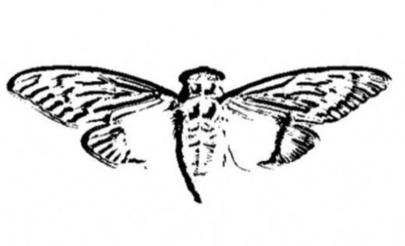
\includegraphics[width=3.00cm]{img/cicada3301/Cicada_3301_logo.jpg}~\\
			\texttt{\scriptsize https://fr.wikipedia.org/wiki/Cicada\_3301}
		\end{column}
		\begin{column}[T]{5.05cm}
			\begin{itemize}
				\footnotesize 
				\item Dixit Wikipedia : ~\\
					"\emph{Cicada 3301 (de l'anglais cicada voulant dire cigale) est une s{\'e}rie de d{\'e}fis organis{\'e}e sur Internet et mettant en jeu {\`a} titre principal des comp{\'e}tences en cryptographie et en informatique. Une s{\'e}rie nouvelle de d{\'e}fis a {\'e}t{\'e} lanc{\'e}e chaque ann{\'e}e autour du 5 janvier en 2012, 2013, 2014 et 2016, dans le but affich{\'e} de recruter 'des individus tr{\`e}s intelligents'. L'identit{\'e} des personnes ou organisations qui organisent ces d{\'e}fis demeure inconnue.}"
				%% \item Cicada3301 Reprend un certain nombre des codes des ARG, mais le quatri{\`e}me mur n'est pas tomb{\'e}...
			\end{itemize}
			%% 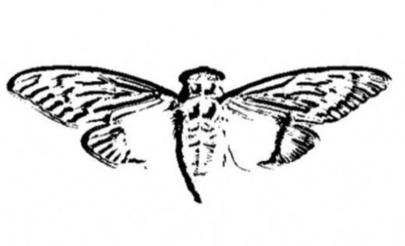
\includegraphics[width=3.00cm]{img/cicada3301/Cicada_3301_logo.jpg}~\\
		\end{column}
	\end{columns}
\end{frame}

\end{document}
